% ══════════════════════════════════════════════════════════════════════
% CHAPTER 6: VISUALISATION MODES
% ══════════════════════════════════════════════════════════════════════

\chapter{Visualisation Modes}
\label{ch:visualisation}

Seismic Viewer provides four primary visualisation modes, each addressing a distinct analytical need. This chapter documents their implementation, rendering strategies, and integration with auxiliary geophysical data layers.

\section{2D Geospatial Map View}
\label{sec:view-2d}

The 2D view provides a plan-view representation of earthquake epicentres overlaid on OpenStreetMap \cite{openstreetmap} tiles, implemented through Plotly's map interfaces (\texttt{scatter\_map} and \texttt{scatter\_mapbox}). The map visualises seismic data using two distinct graphical layers:
\begin{itemize}
    \item \textbf{Scatter Markers}: Each earthquake is represented by a circular marker. The visual properties of these circles can be mapped to different physical parameters depending on analytical needs. By default, the size of the circle indicates the magnitude of the event (with a minimum size threshold to ensure micro-earthquakes remain visible), and the colour represents the hypocentral depth. These mappings are flexible, allowing users to visualise other variables, such as chronological progression. Users can interact with these markers by hovering over them to reveal detailed statistics.
    \item \textbf{Density Heatmap}: A spatial density layer that visually aggregates tightly clustered earthquakes. By rendering a continuous colour gradient over regions of high seismicity, this optional overlay allows researchers to identify active swarm locations and broader structural trends that might be difficult to perceive when analysing individual scatter points alone.
\end{itemize}

To explore the dataset, users can apply filters based on magnitude, depth, and date ranges using dedicated input fields located on the left-hand panel. All filtering operations are processed directly within the user's web browser. This approach avoids sending new requests to the main server, ensuring that the map updates promptly whenever a parameter is changed.

\begin{figure}[H]
\centering
\begin{subfigure}[t]{0.85\textwidth}
\centering
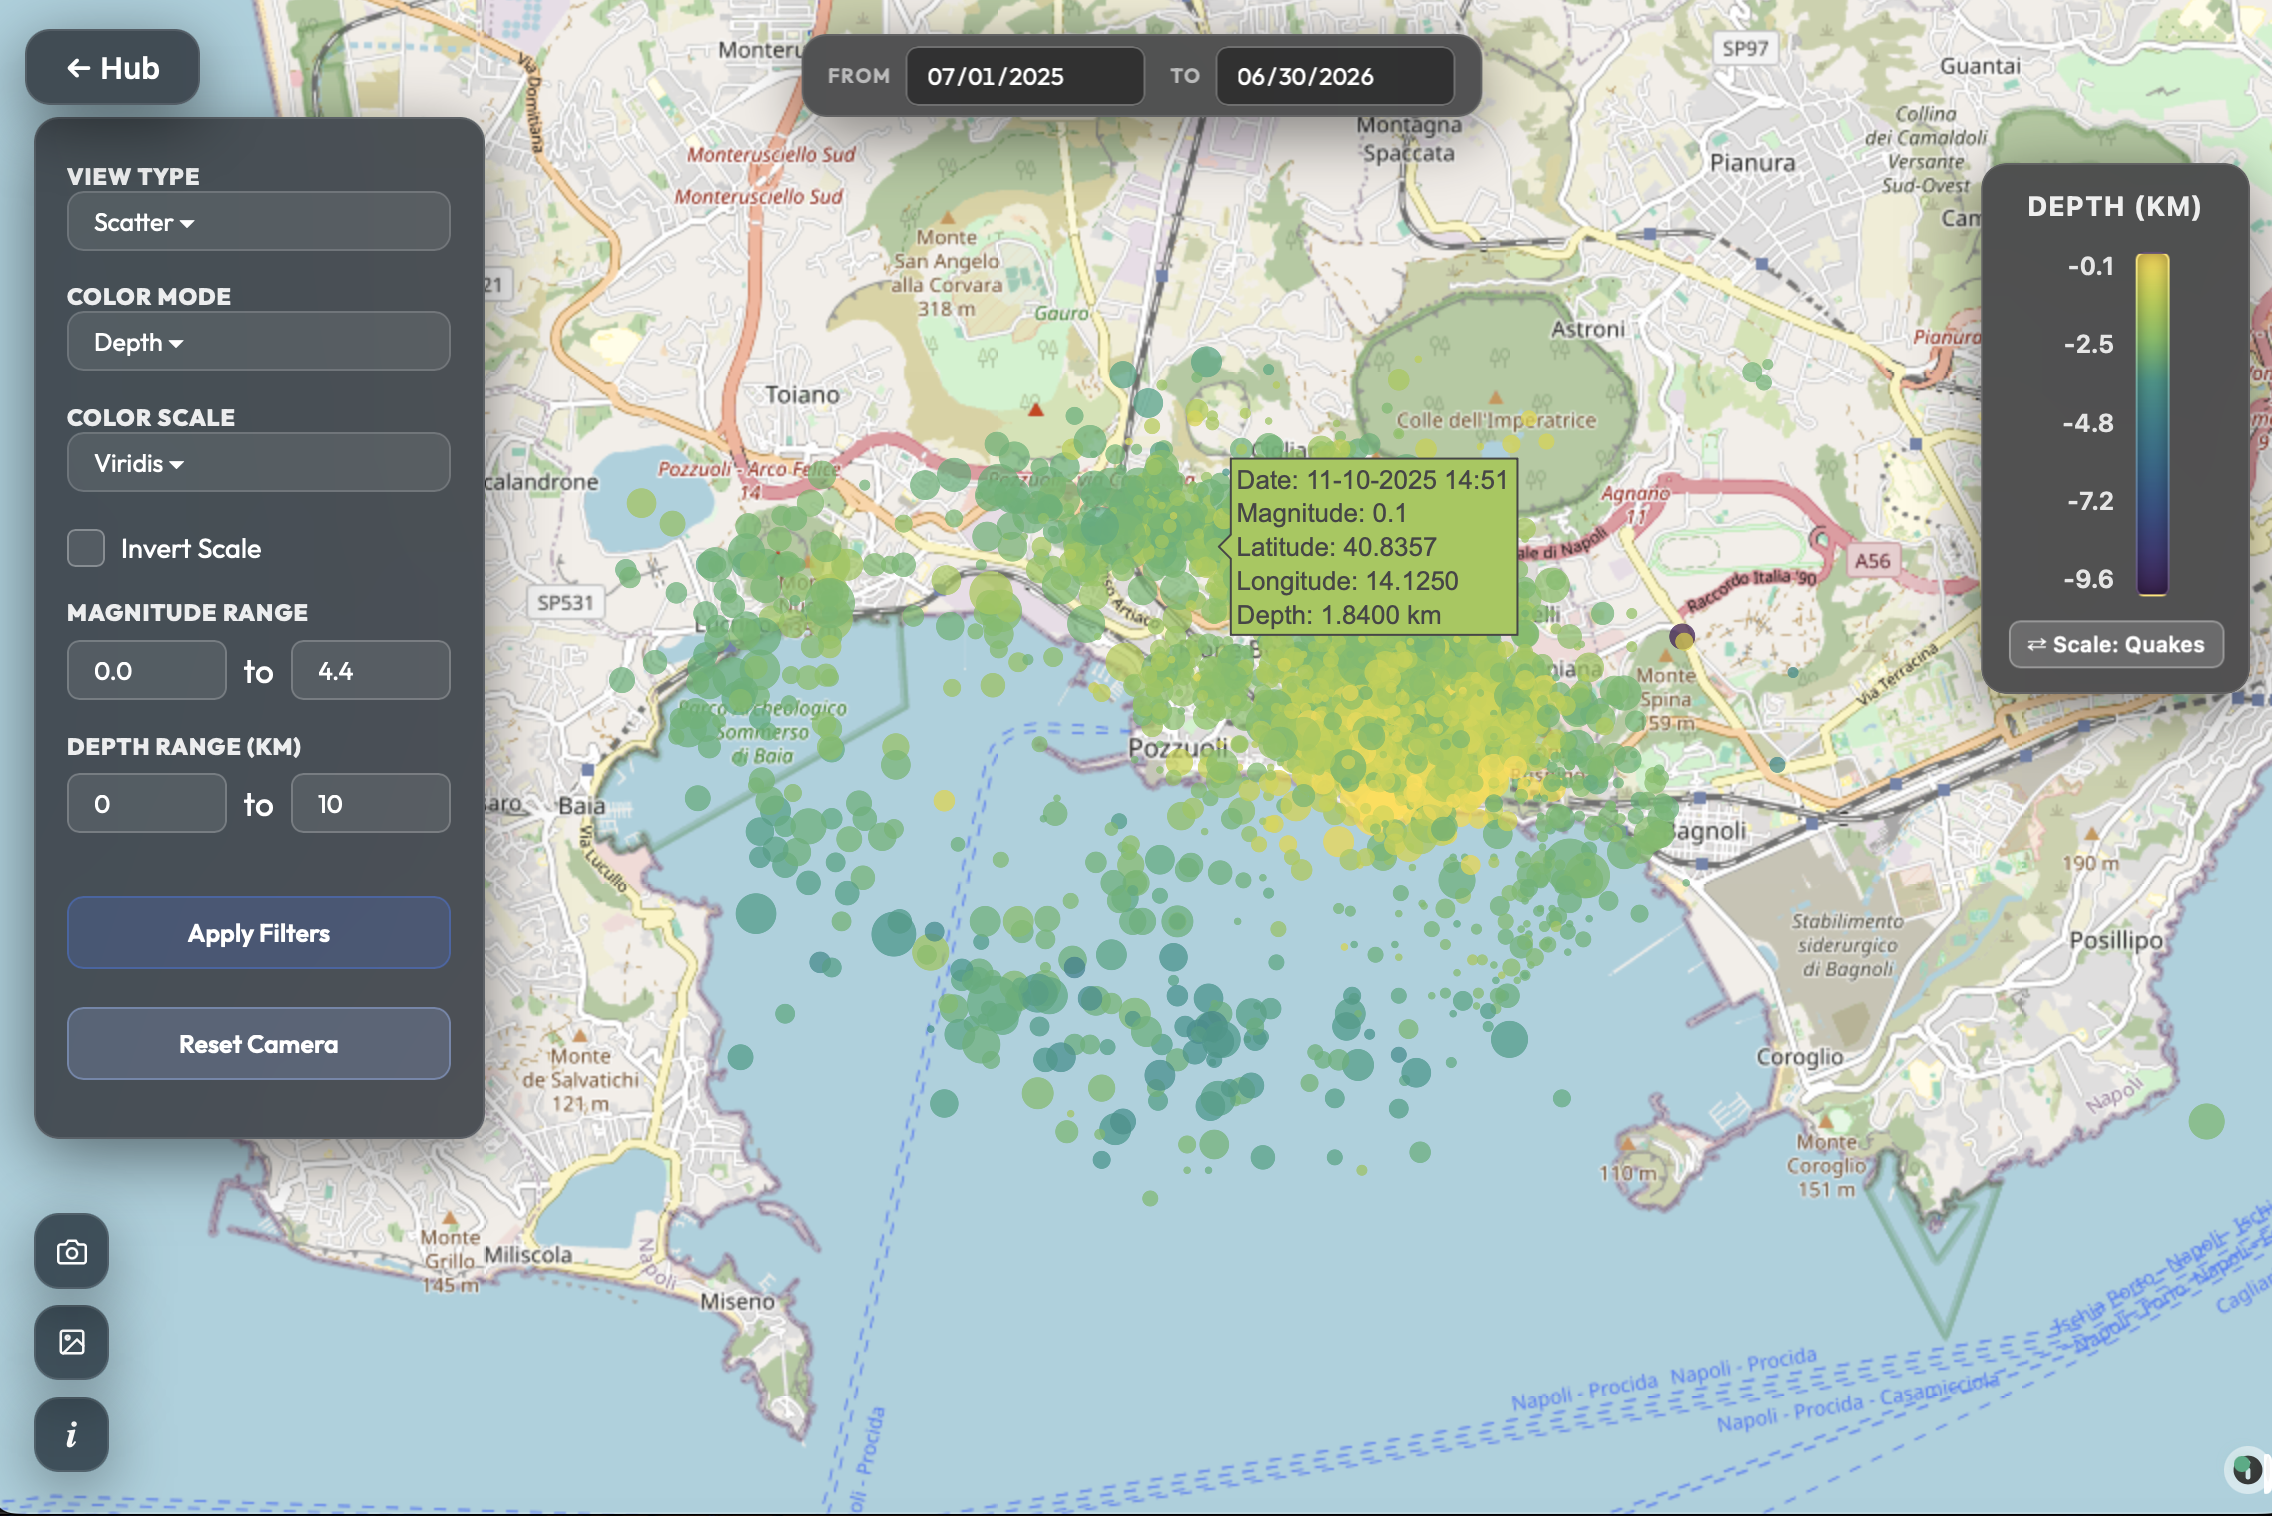
\includegraphics[width=\textwidth, height=0.66\textwidth]{images/2d_visualization.png}
\caption{The 2D base map showing earthquake locations. On the left panel, input fields allow the user to filter the data by magnitude, depth, and date.}
\label{fig:2d-viz}
\end{subfigure}
\end{figure}

\begin{figure}[H]
\ContinuedFloat
\centering
\begin{subfigure}[t]{0.85\textwidth}
\centering
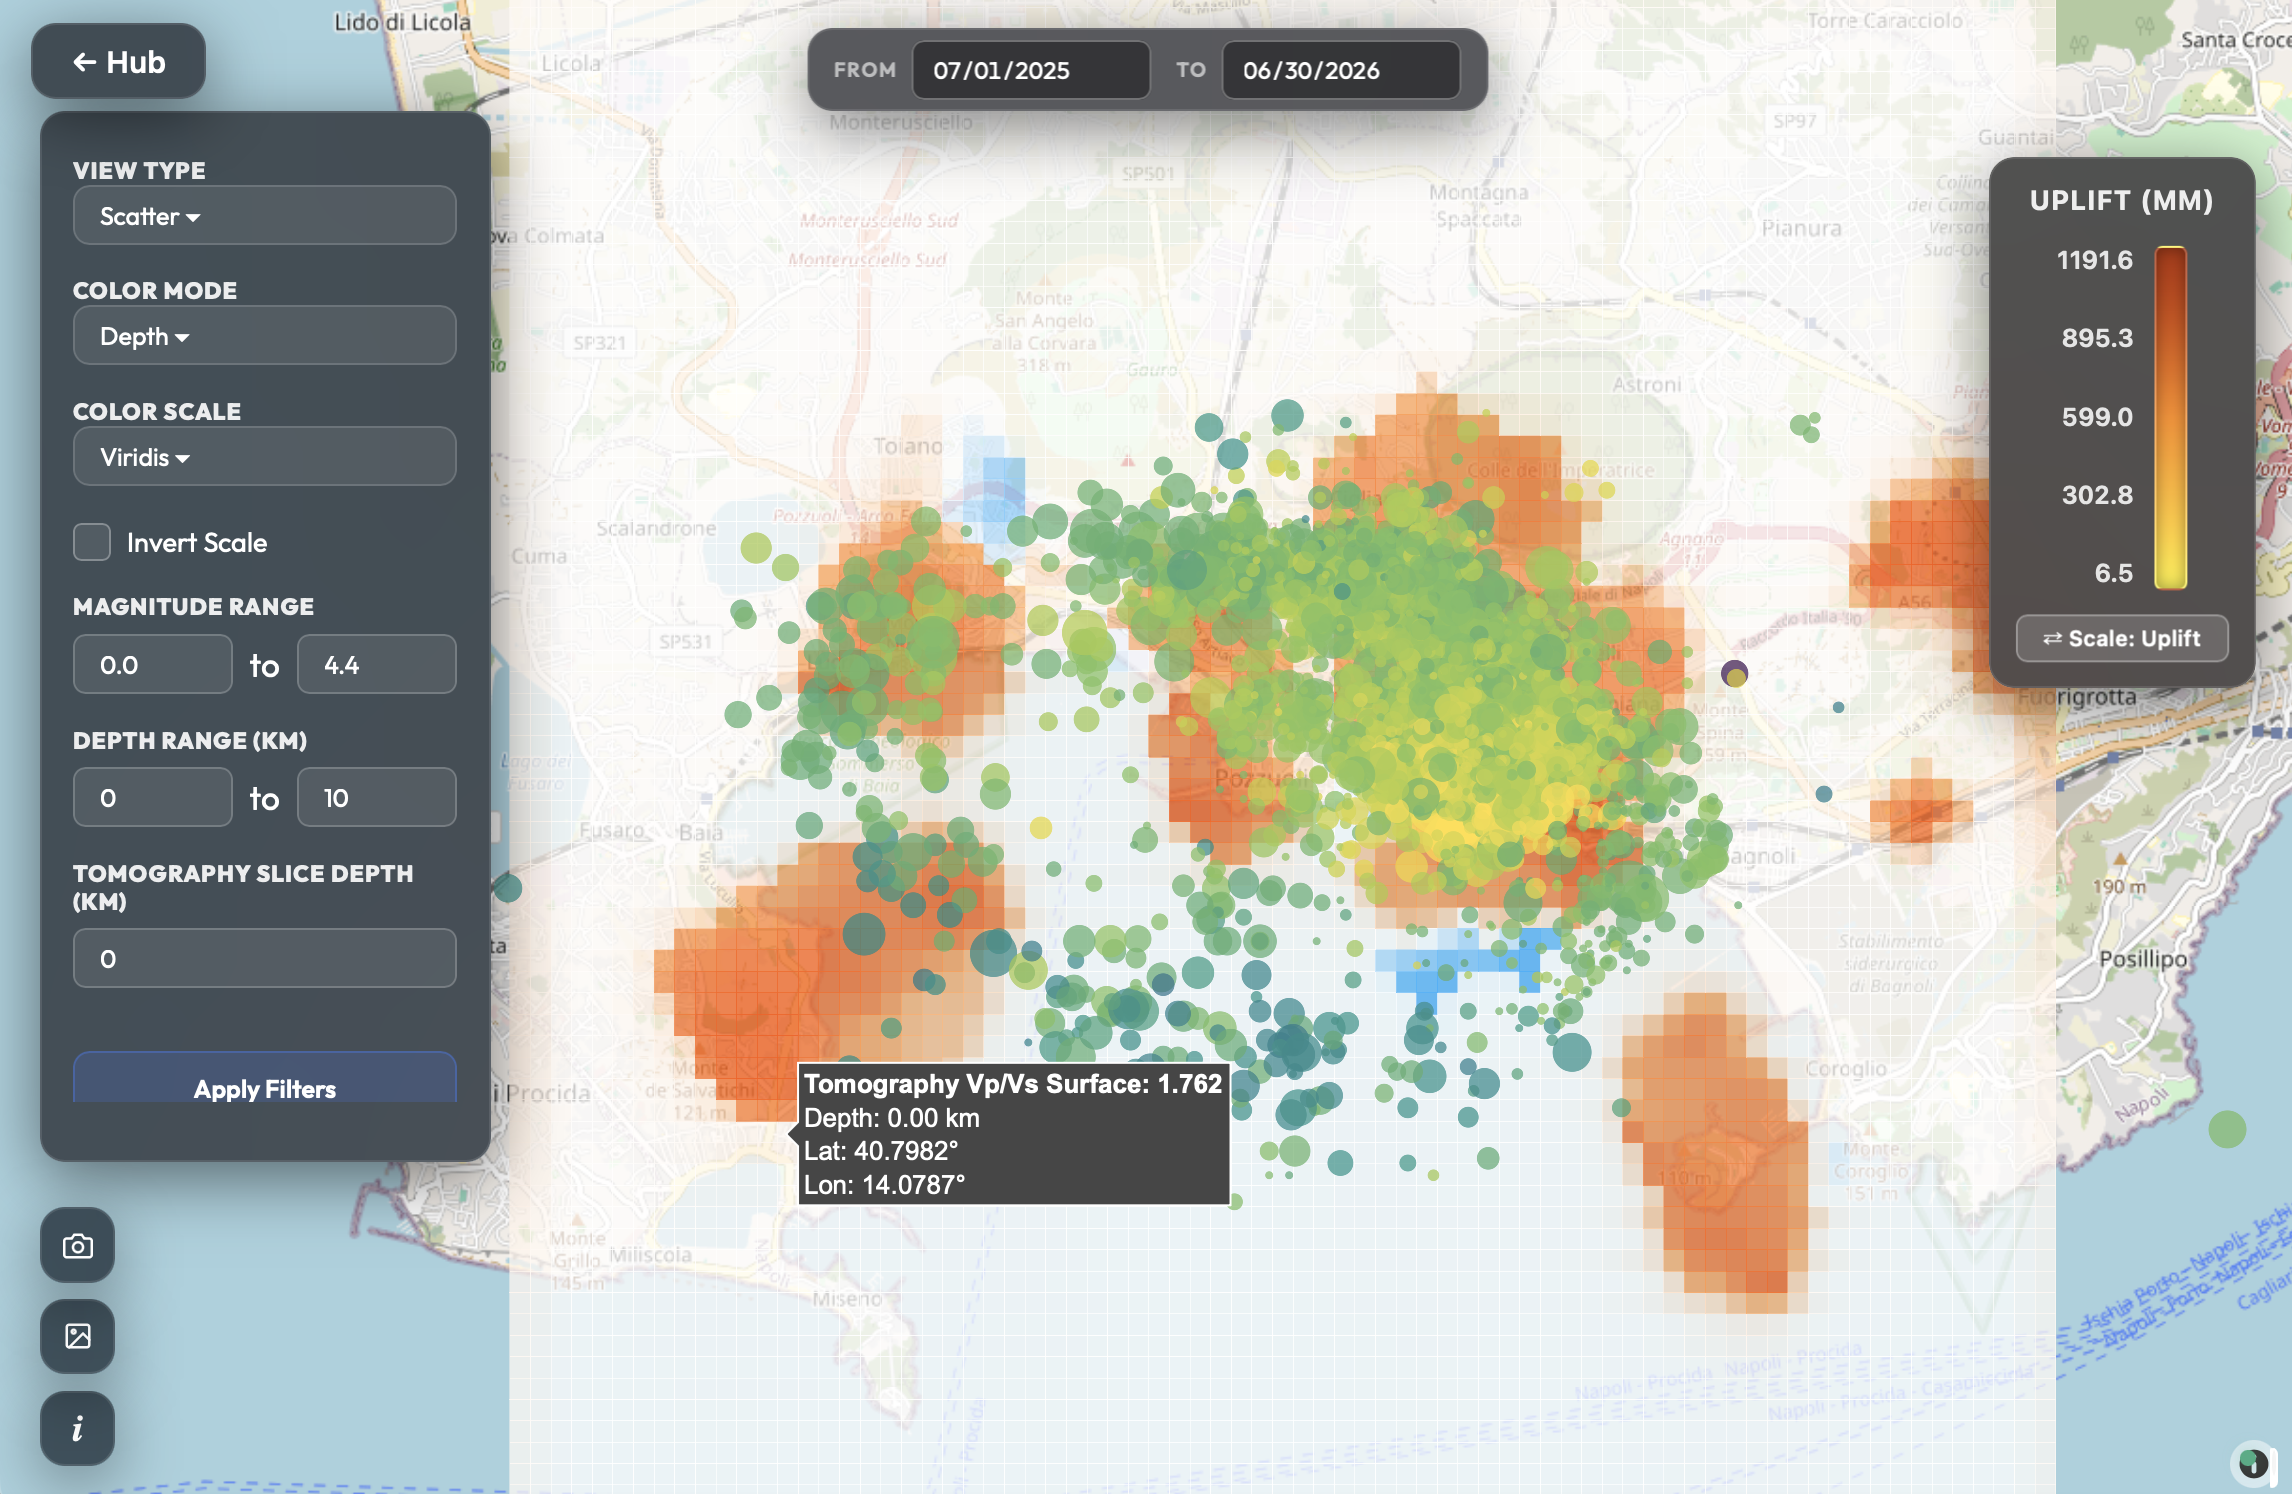
\includegraphics[width=\textwidth, height=0.66\textwidth]{images/2d_visualization_tomography.png}
\caption{An overlay showing a tomography slice of the crust. The highlighted areas indicate high $V_p/V_s$ velocity anomalies.}
\label{fig:2d-viz-tomo}
\end{subfigure}
\end{figure}

\begin{figure}[H]
\ContinuedFloat
\centering
\begin{subfigure}[t]{0.85\textwidth}
\centering
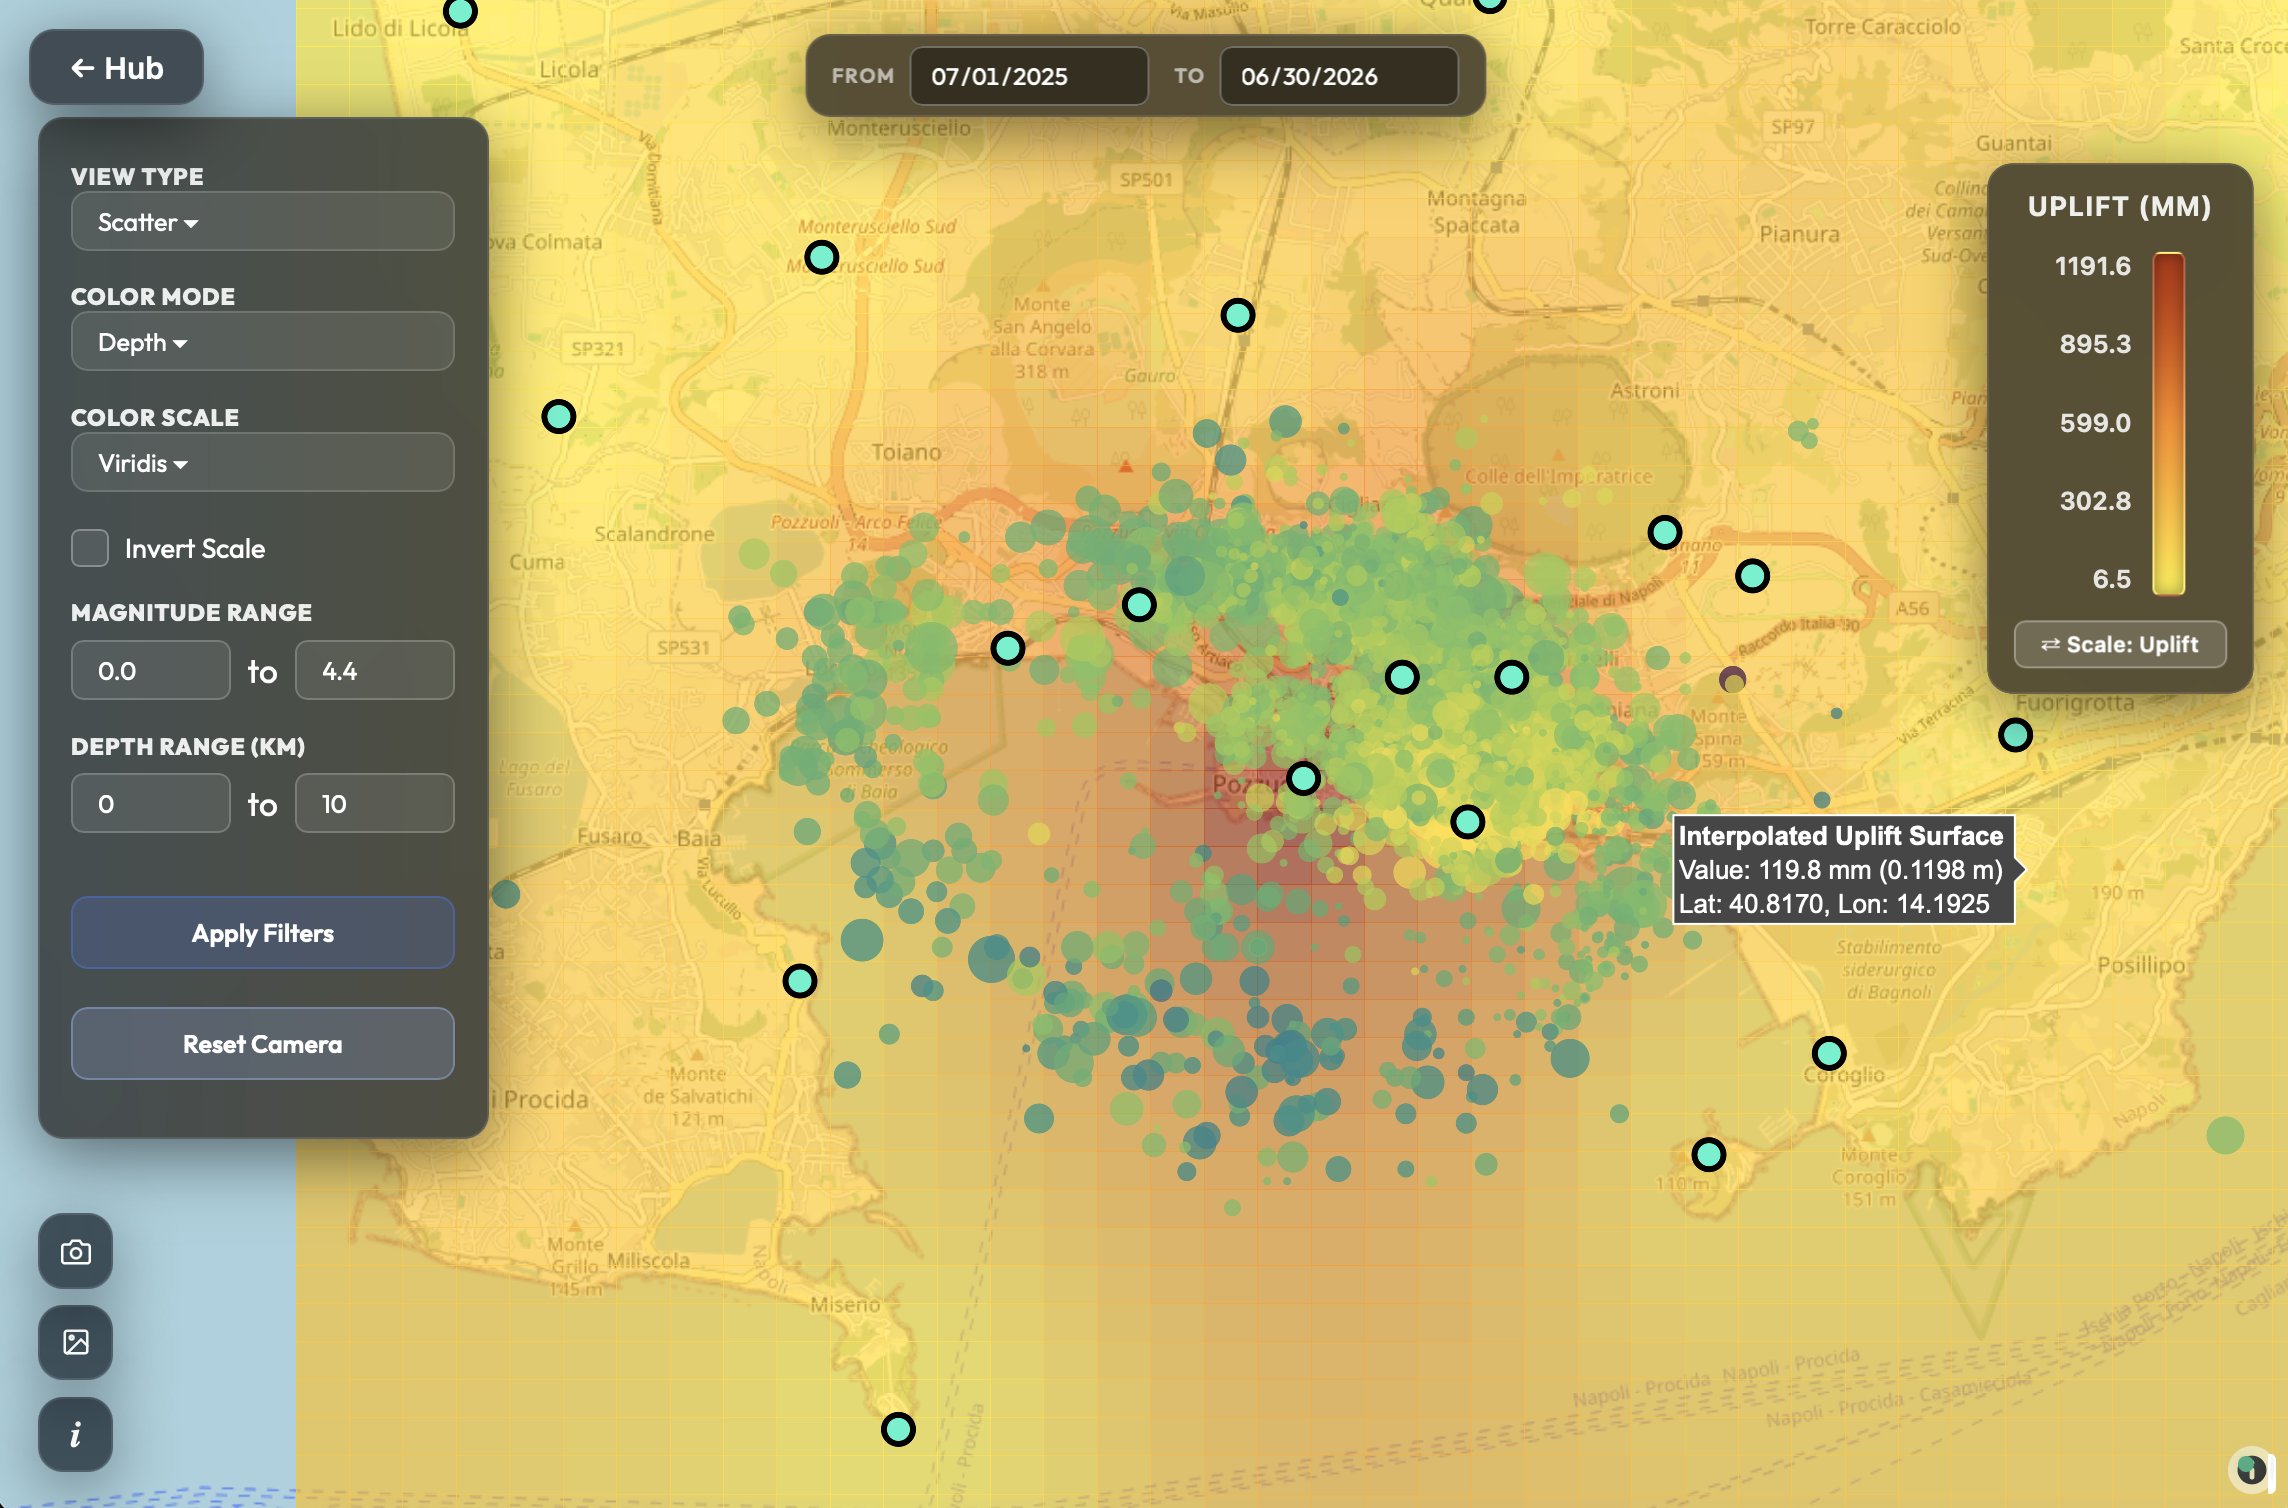
\includegraphics[width=\textwidth]{images/2d_visualization_uplift_stations.png}
\caption{An overlay displaying vertical ground movement (uplift) using a grid map, along with the locations of permanent monitoring stations across Campi Flegrei.}
\label{fig:2d-viz-uplift}
\end{subfigure}
\caption{The 2D Geospatial Map View in the Seismic Viewer. This workspace allows users to filter earthquake data (\subref{fig:2d-viz}) and combine it with advanced geophysical overlays, such as tomographic velocity maps (\subref{fig:2d-viz-tomo}) and ground uplift measurements (\subref{fig:2d-viz-uplift}).}
\label{fig:2d-multi}
\end{figure}

As shown in \Cref{fig:2d-multi}, the 2D workspace offers three visualisation options. The base view (\Cref{fig:2d-viz}) displays earthquake locations on an OpenStreetMap layer, while the side panel allows users to filter events by magnitude, depth, and date. In \Cref{fig:2d-viz-tomo}, a tomographic slice shows variations in the $V_p/V_s$ velocity ratio, indicating underground fluid bodies. Finally, in \Cref{fig:2d-viz-uplift}, the map combines monitoring stations with vertical ground movement, helping researchers observe if earthquakes match areas of surface uplift.

\section{3D Static View}
\label{sec:view-3d-static}

The 3D static view renders hypocentres as a subsurface point cloud within a three-dimensional geographic volume beneath an OpenStreetMap terrain surface. The reference terrain is rendered as a flat, unshaded map layer for clarity, while earthquakes are represented beneath the surface as a 3D point cloud, colour-coded by variables like depth or time.

To prevent geographic distortion caused by Earth's sphericity, the system scales horizontal proportions based on latitude:
\begin{equation}
    \text{ratio}_x = \frac{\Delta\lambda \cdot K \cdot \cos(\bar{\phi})}{\max(d_\text{lon}, d_\text{lat})}, \quad
    \text{ratio}_y = \frac{\Delta\phi \cdot K}{\max(d_\text{lon}, d_\text{lat})}
    \label{eq:aspect-ratio}
\end{equation}
where $\Delta\lambda$ and $\Delta\phi$ are the longitude and latitude spans, $K = 111.32$~km/° is the equatorial conversion factor, and $\bar{\phi}$ is the mean latitude. This adjustment preserves accurate spatial proportions.

Rendering large point clouds simultaneously relies on GPU acceleration. Plotly.js uses WebGL to draw points via the \texttt{scatter3d} trace type. To maintain smooth interactive frame rates, the application applies three measures: (1) map background images are scaled to save memory, (2) automatic bounding box recalculations are disabled during updates, and (3) markers are drawn as point sprites facing the camera rather than complex 3D shapes.

As shown in \Cref{fig:3d-multi}, the 3D static workspace presents these data layers in three dimensions. The base view (\Cref{fig:3d-viz}) shows hypocentres below the map surface, using colours to represent depth intervals. In \Cref{fig:3d-viz-tomo}, the scene adds velocity slices from the tomography model. Finally, in \Cref{fig:3d-viz-uplift}, vertical columns indicate surface movement at each station, allowing direct comparisons between depth and surface observations.

\begin{figure}[H]
\centering
\begin{subfigure}[t]{1.0\textwidth}
\centering
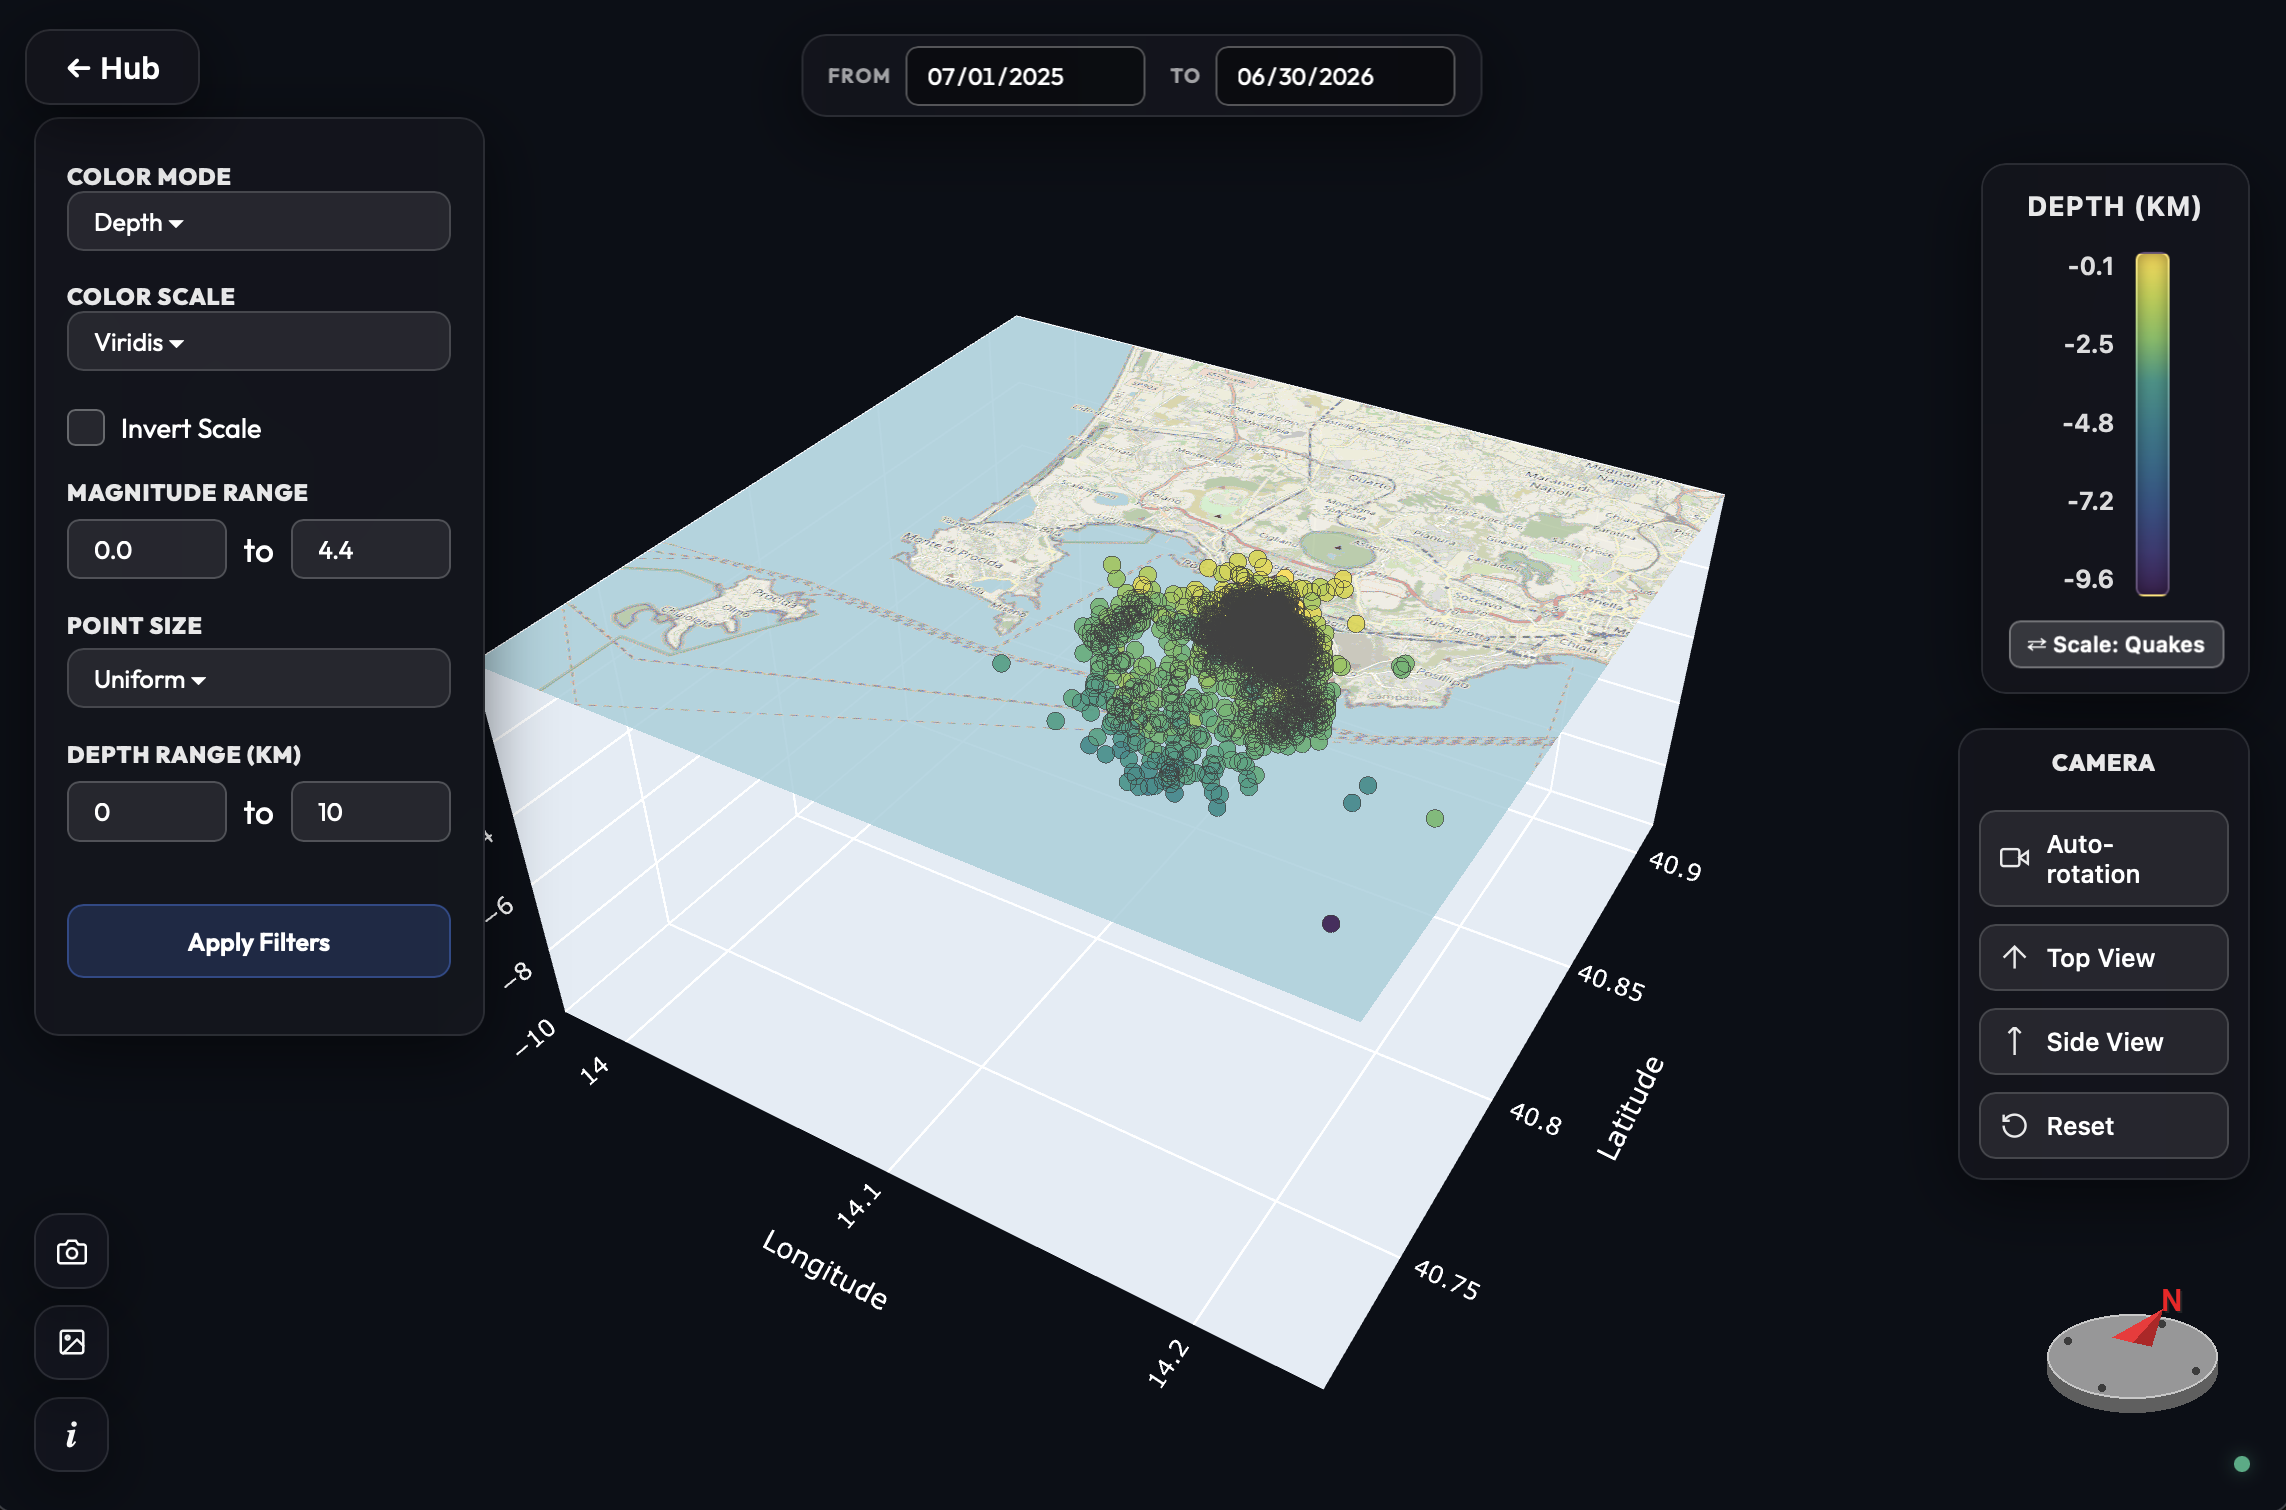
\includegraphics[width=\textwidth]{images/3d_visualization.png}
\caption{Point cloud below surface map.}
\label{fig:3d-viz}
\end{subfigure}
\end{figure}

\begin{figure}[H]
\ContinuedFloat
\centering
\begin{subfigure}[t]{1.0\textwidth}
\centering
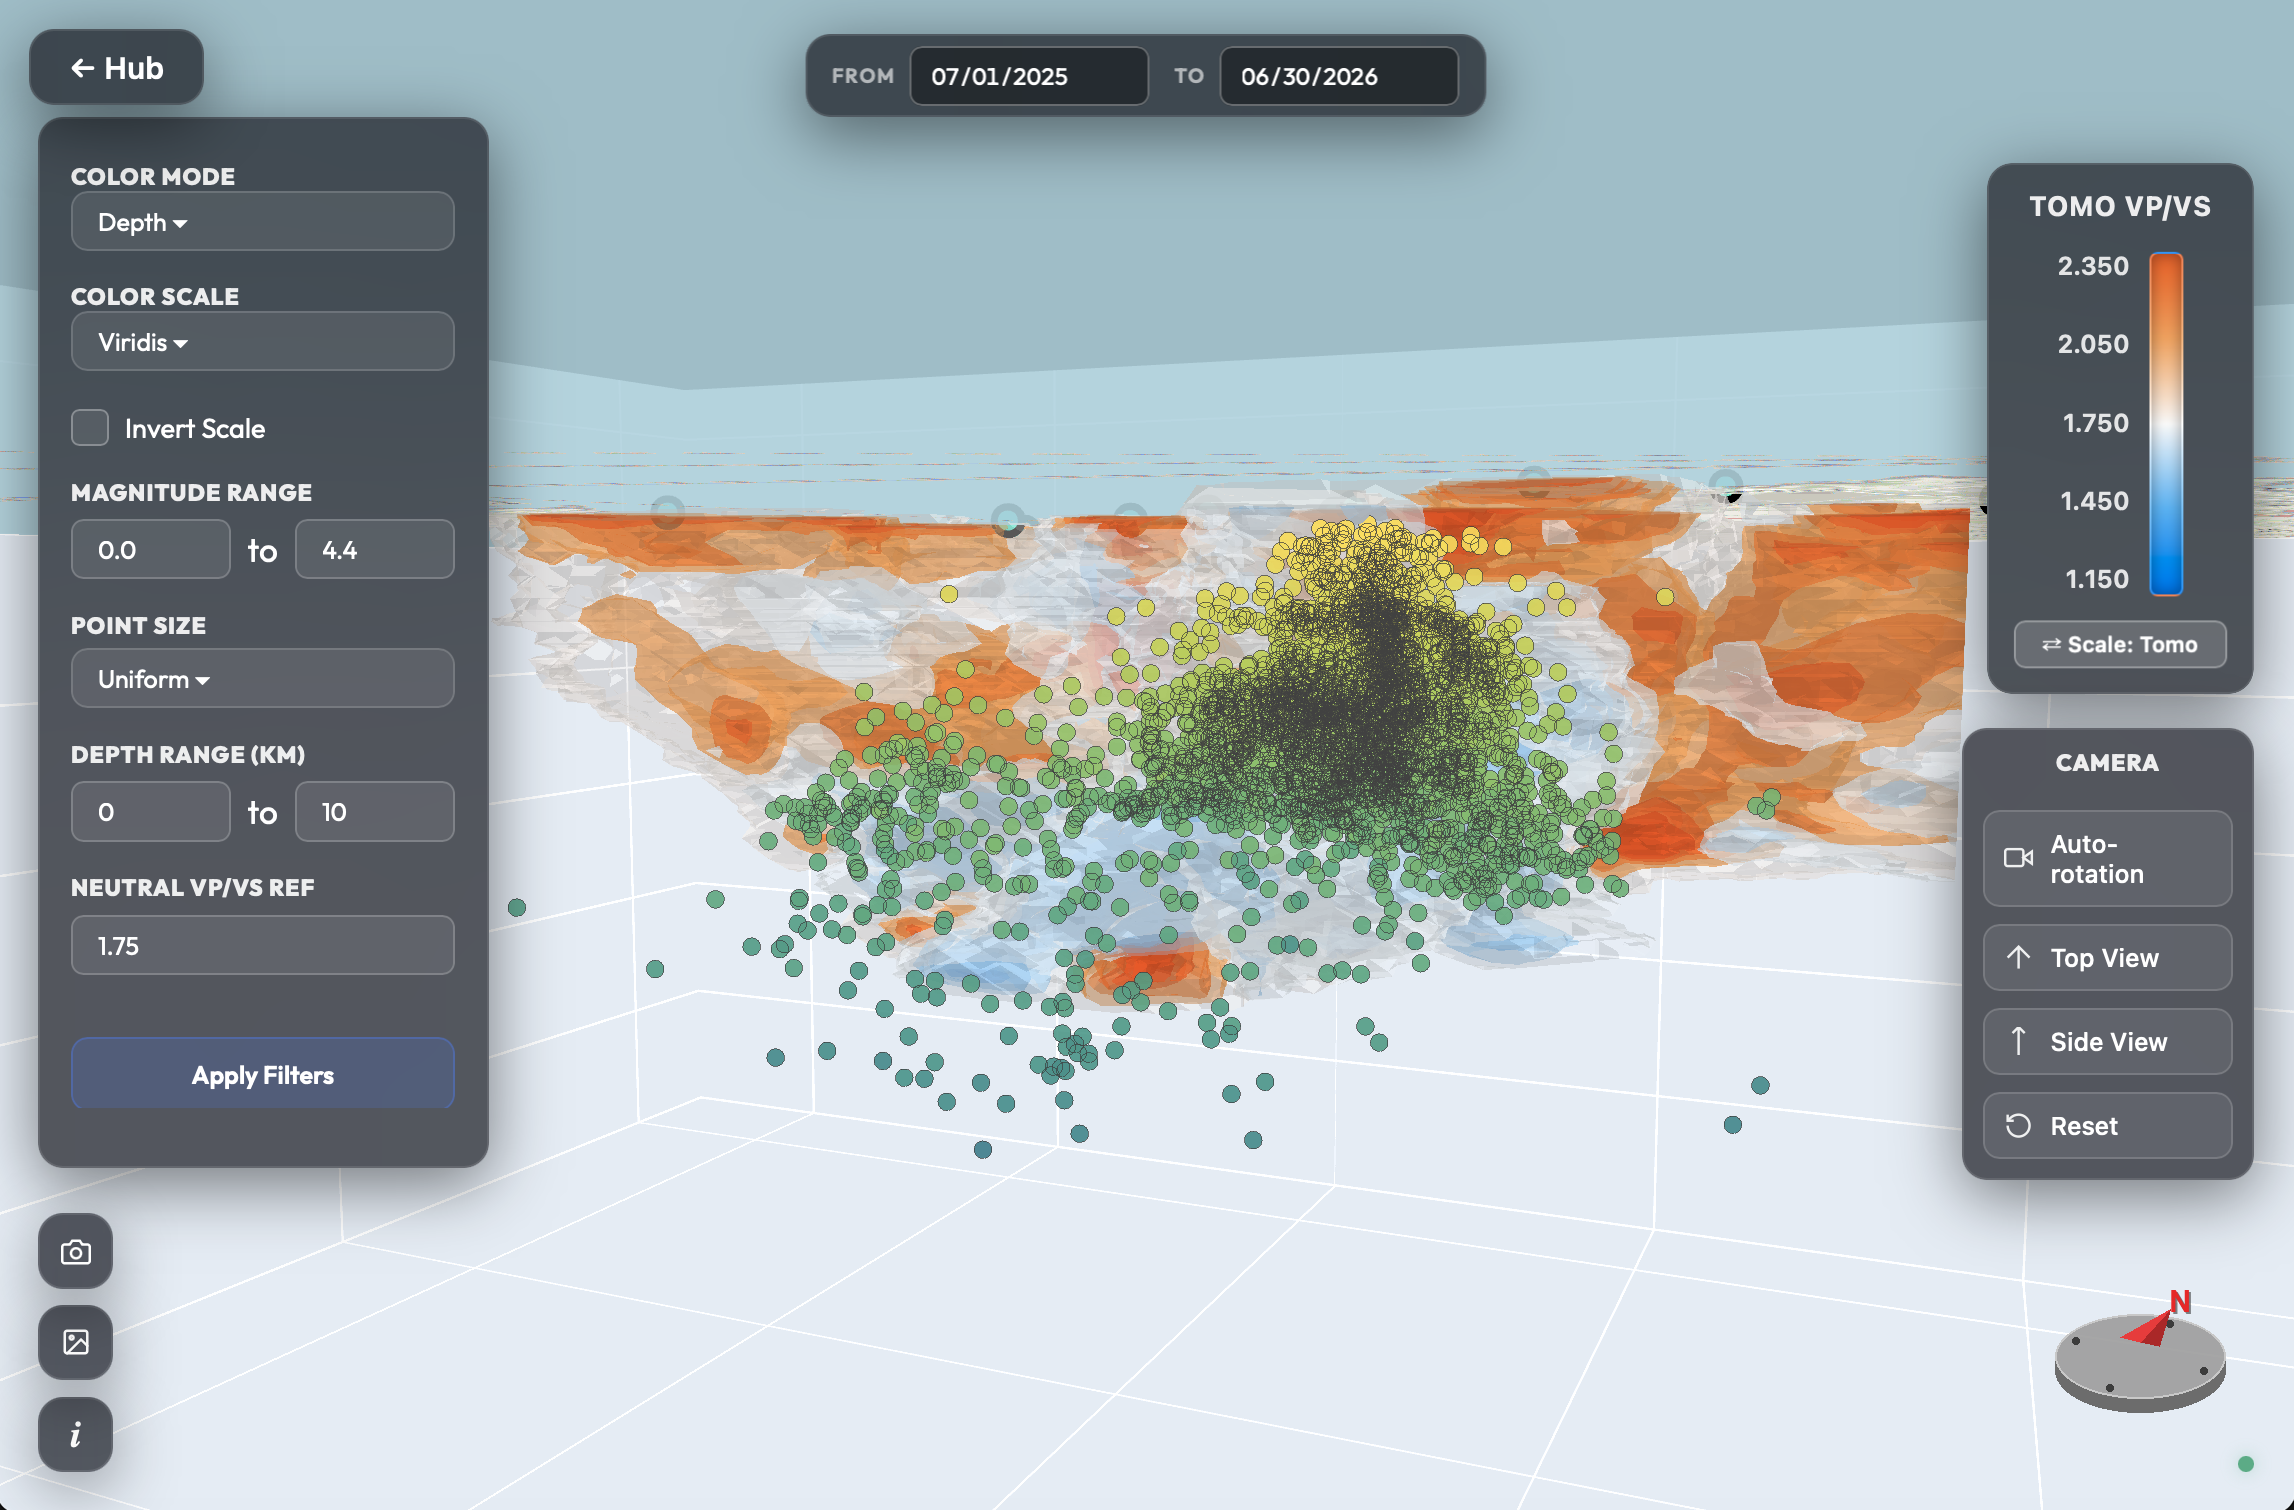
\includegraphics[width=\textwidth]{images/3d_visualization_tomography.png}
\caption{Added tomography layer.}
\label{fig:3d-viz-tomo}
\end{subfigure}
\end{figure}

\begin{figure}[H]
\ContinuedFloat
\centering
\begin{subfigure}[t]{1.0\textwidth}
\centering
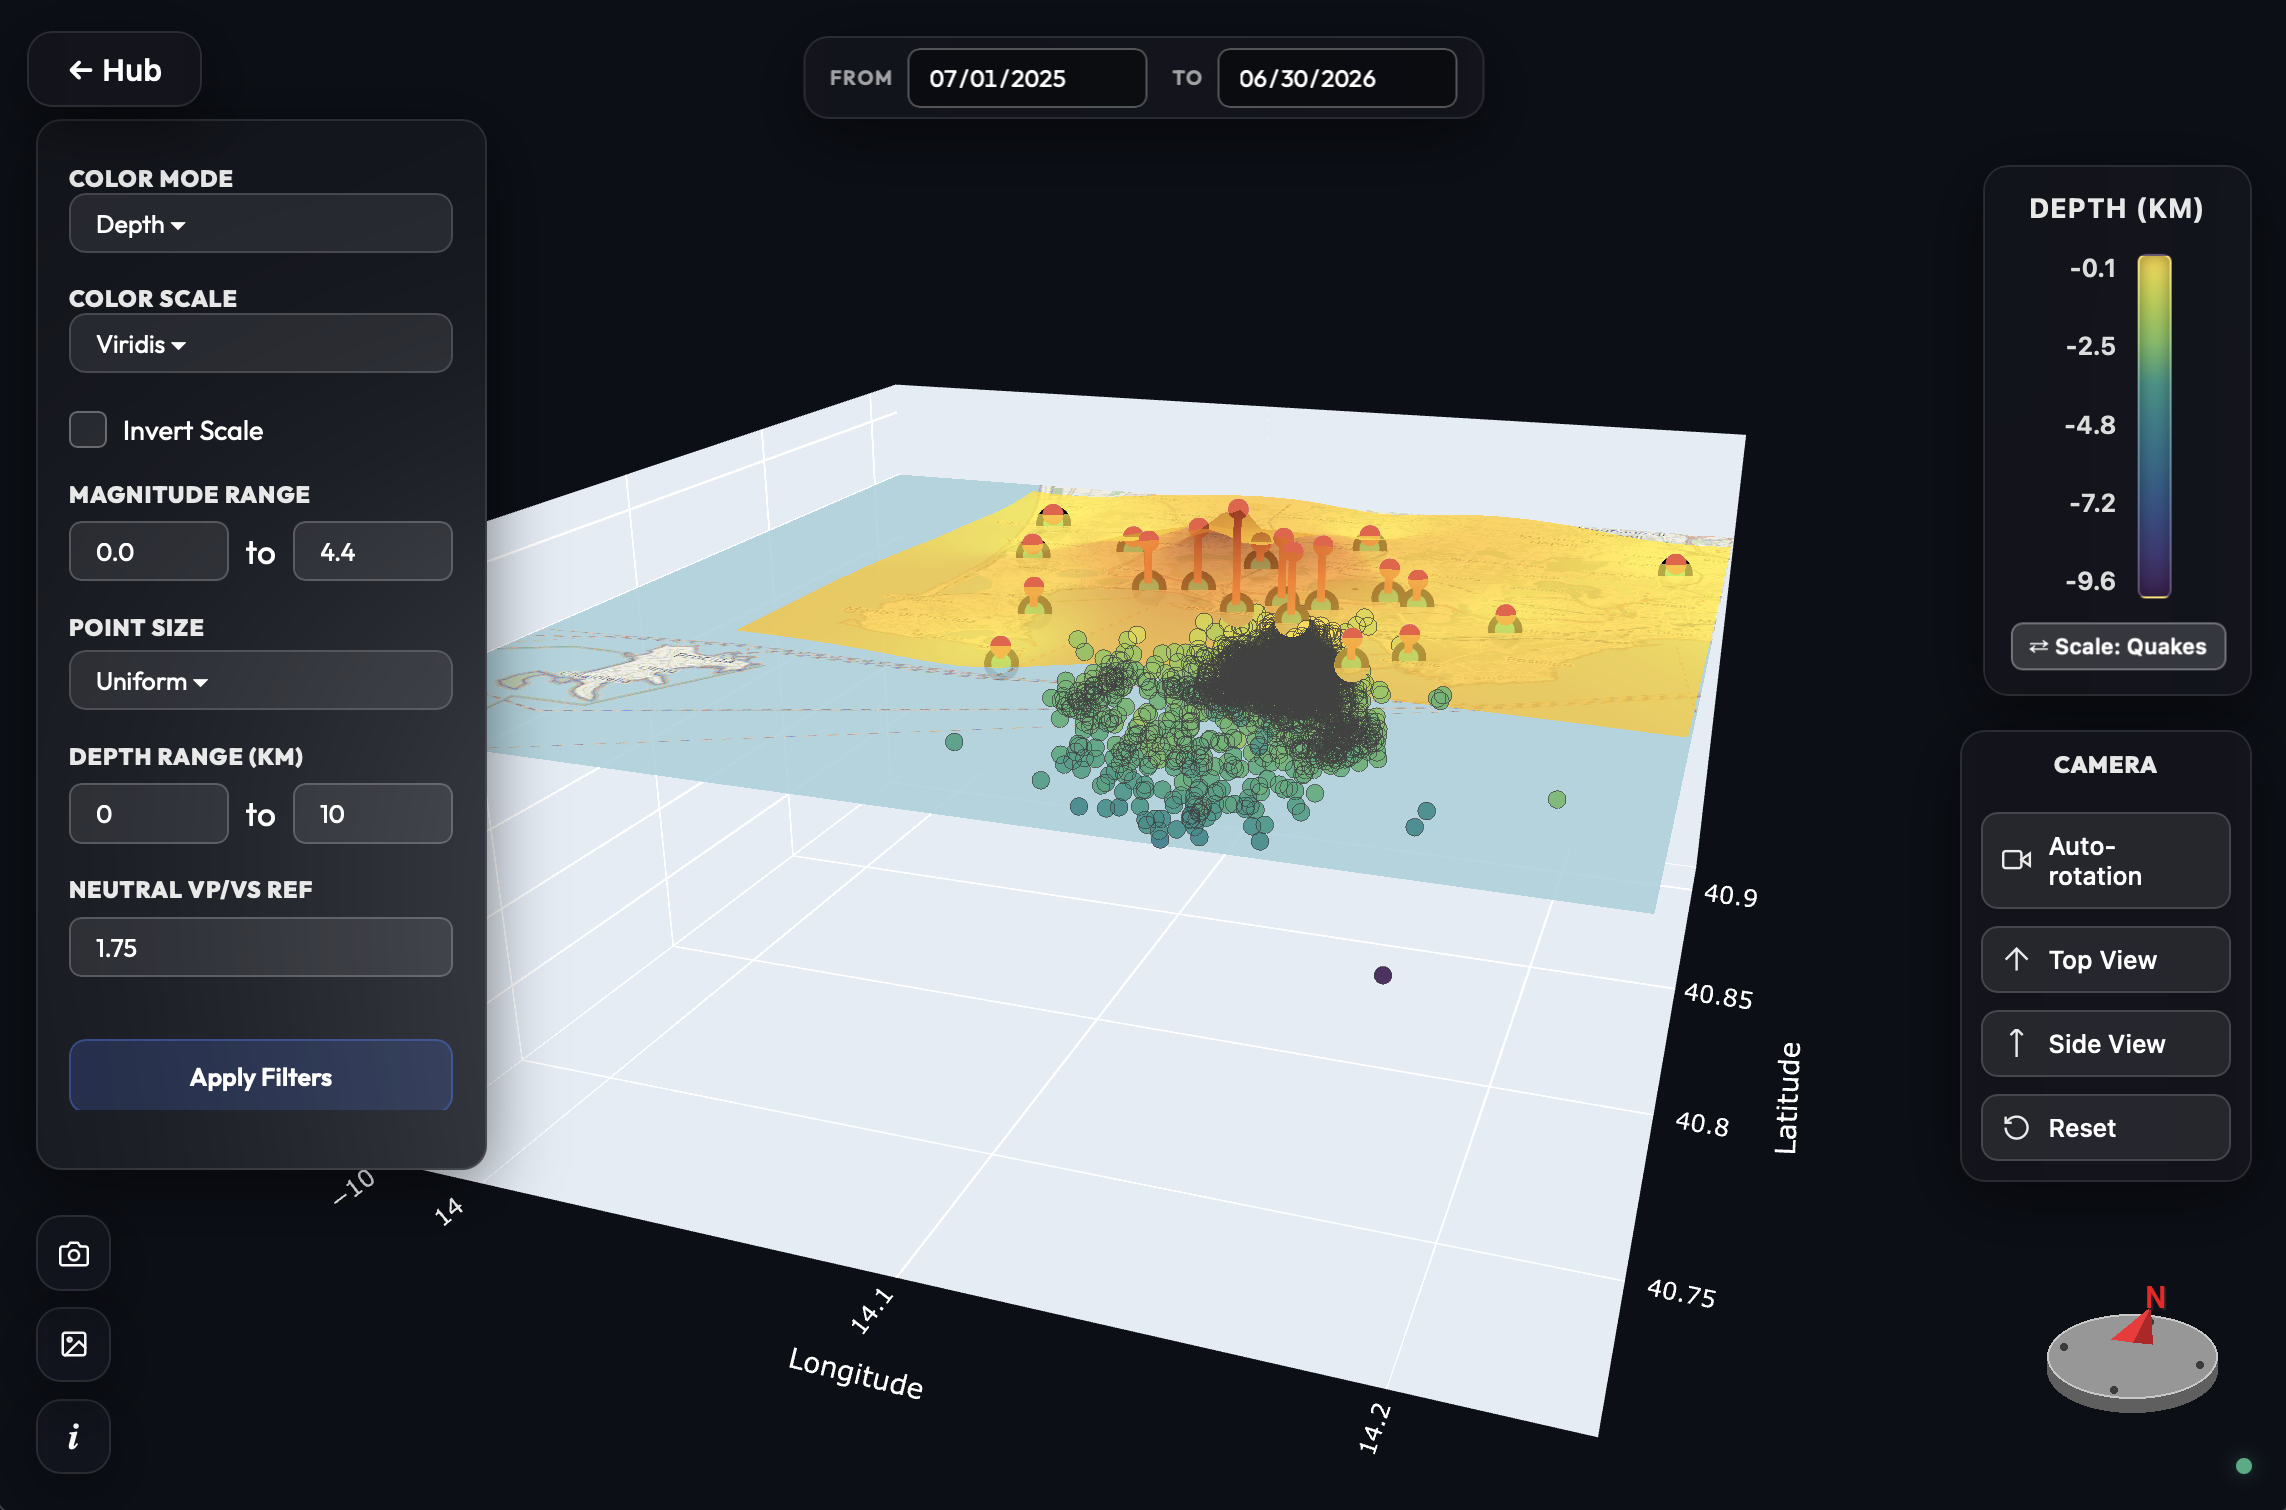
\includegraphics[width=\textwidth]{images/3d_visualization_uplift_stations.png}
\caption{Ground uplift columns.}
\label{fig:3d-viz-uplift}
\end{subfigure}
\caption{The 3D Static View workspace. The user can explore the underground earthquake distribution (\subref{fig:3d-viz}) and combine it with 3D tomography models (\subref{fig:3d-viz-tomo}) and surface deformation data (\subref{fig:3d-viz-uplift}).}
\label{fig:3d-multi}
\end{figure}

\section{3D Animated View (4D Visualisation)}
\label{sec:view-animated}

The animated view adds time as a fourth dimension to observe the spatio-temporal evolution of seismic sequences.

The 4D visualisation engine offers four temporal modes to analyse seismic evolution: \textbf{Accumulation} (showing all events up to the current frame), \textbf{Sliding window} (displaying events within a moving time frame), \textbf{Block mode} (rendering discrete, non-overlapping time intervals), and \textbf{Seismic Swarms} (focusing on episodic bursts identified by automated detection according to INGV criteria, supported by timeline navigation and magnitude or depth charts). To ensure smooth playback and avoid memory overload, the system precomputes temporal indices and updates the 3D scene dynamically without reloading the entire figure.

During 4D animations, the camera angle and zoom level must remain stable across updates. By default, Plotly reinitialises the view on coordinate changes. Setting \texttt{uirevision='constant'} in the layout preserves camera position and orientation across frames, allowing continuous interaction during playback.

\enlargethispage{5cm}

\begin{figure}[H]
\centering
\begin{subfigure}[t]{0.85\textwidth}
\centering
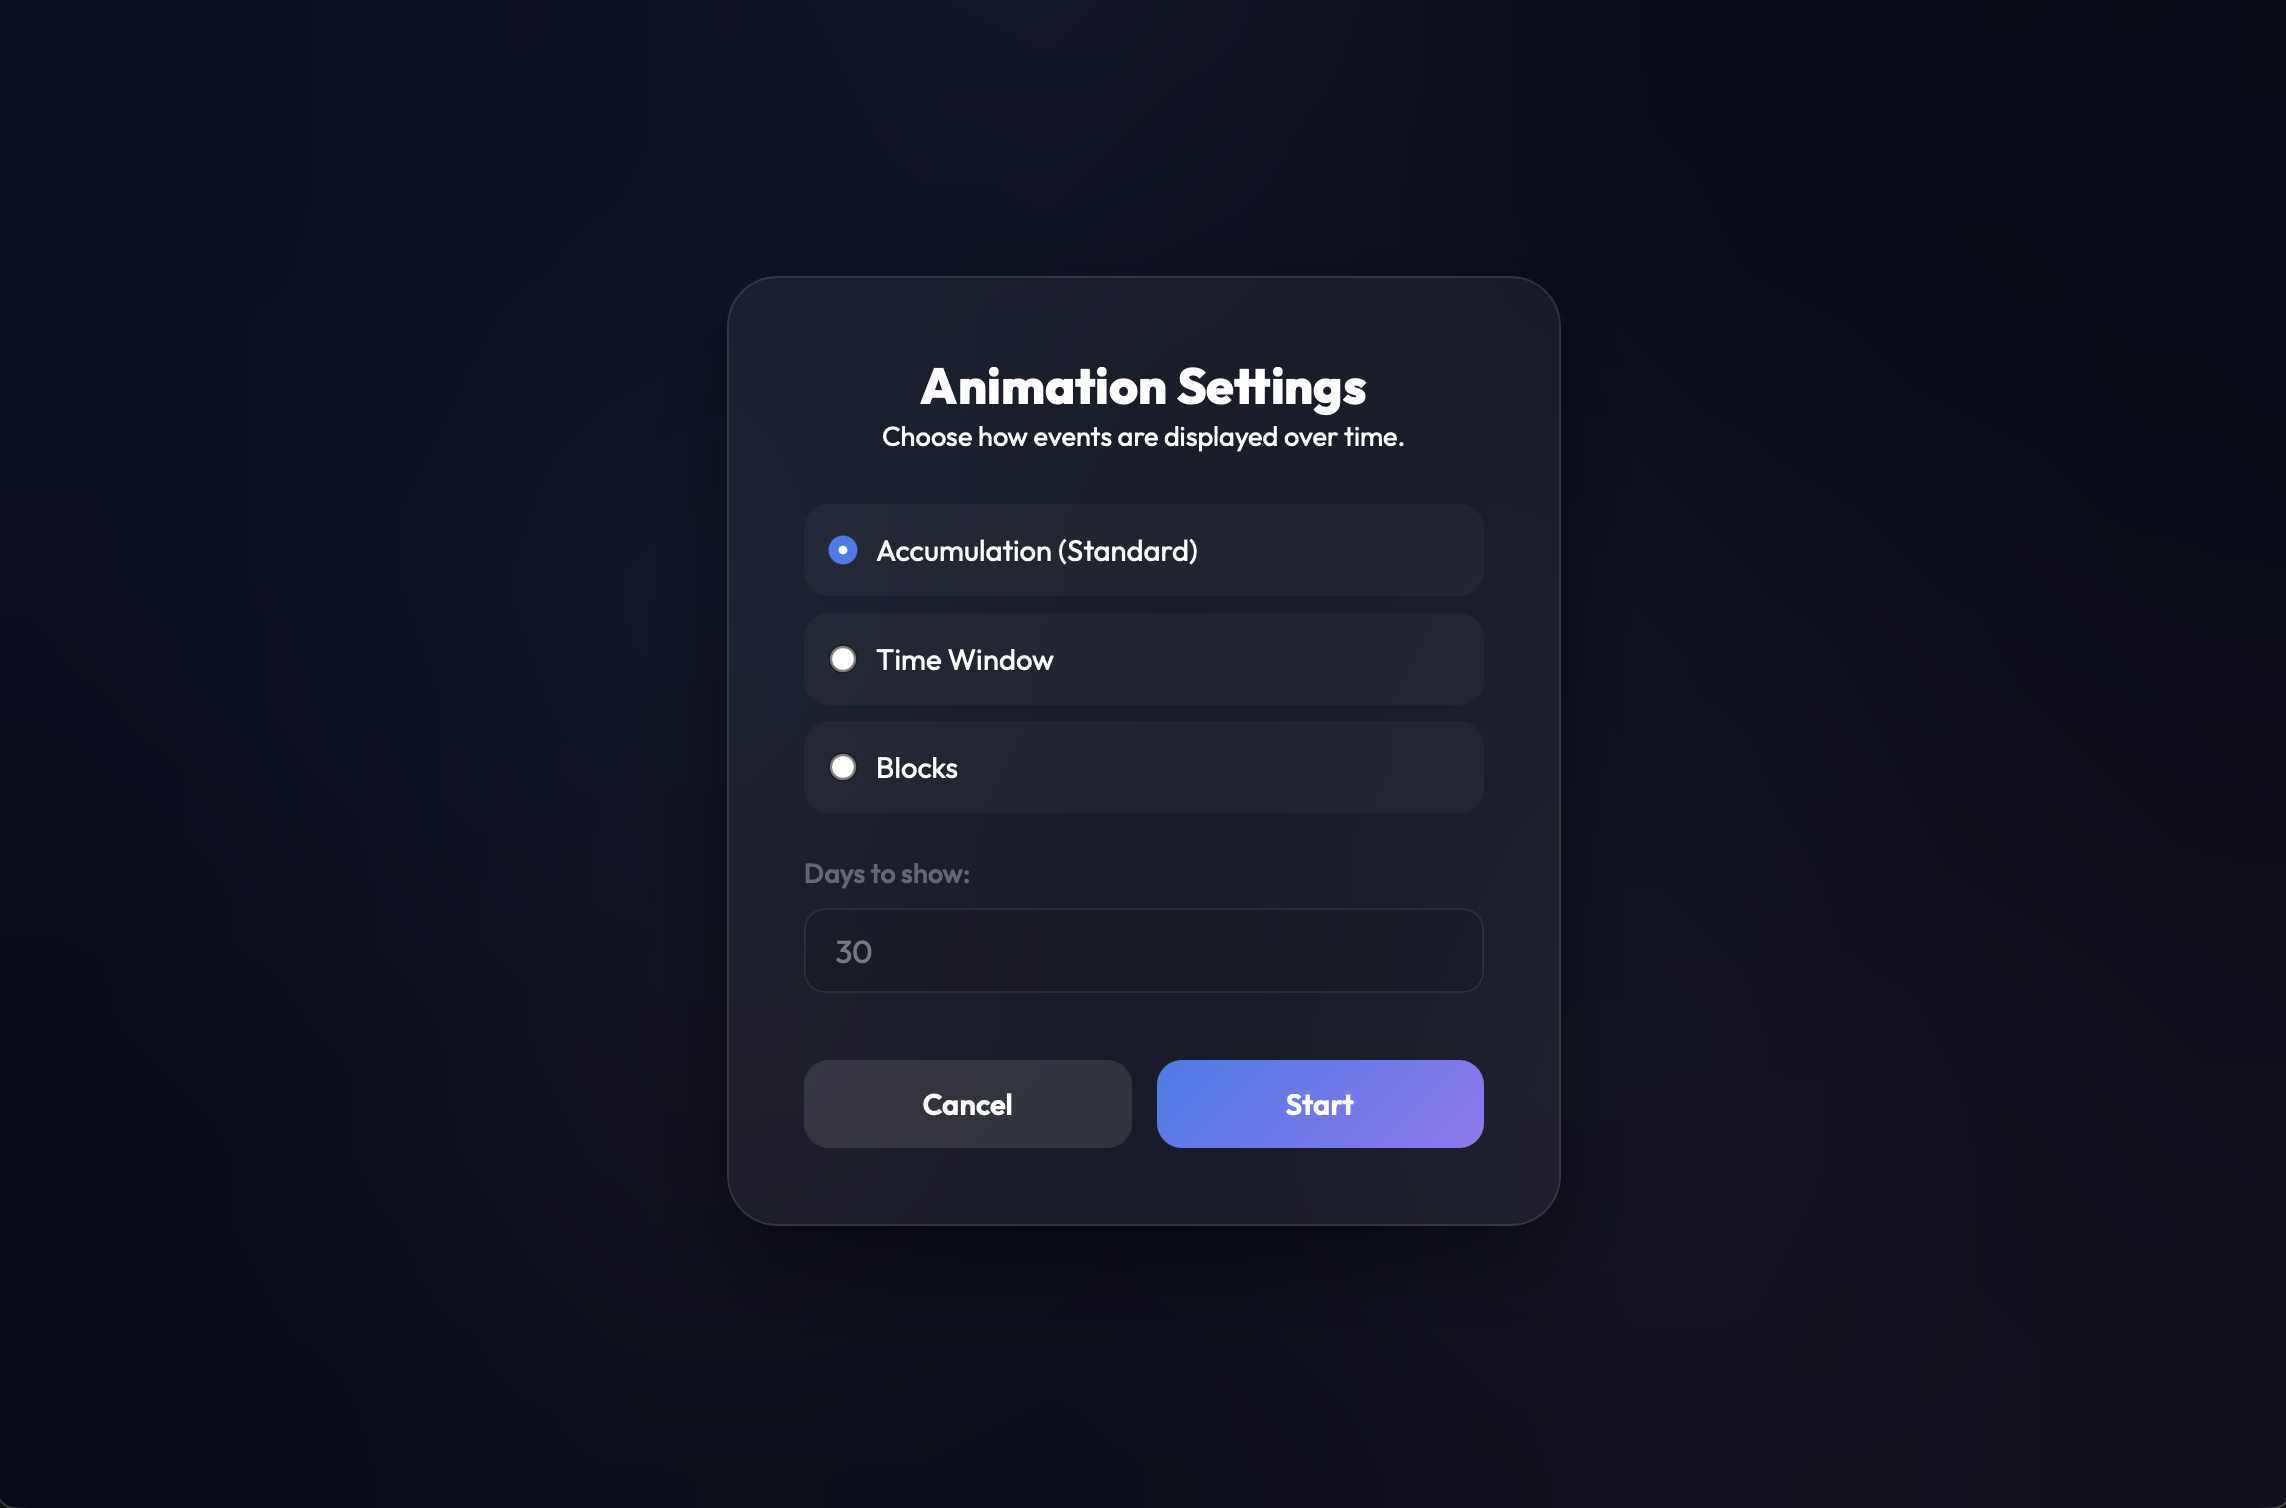
\includegraphics[width=\textwidth]{images/animated_visualization_selection_menu.png}
\caption{Temporal window configuration dialog.}
\label{fig:anim-menu}
\end{subfigure}
\end{figure}

\begin{figure}[H]
\ContinuedFloat
\centering
\begin{subfigure}[t]{0.85\textwidth}
\centering
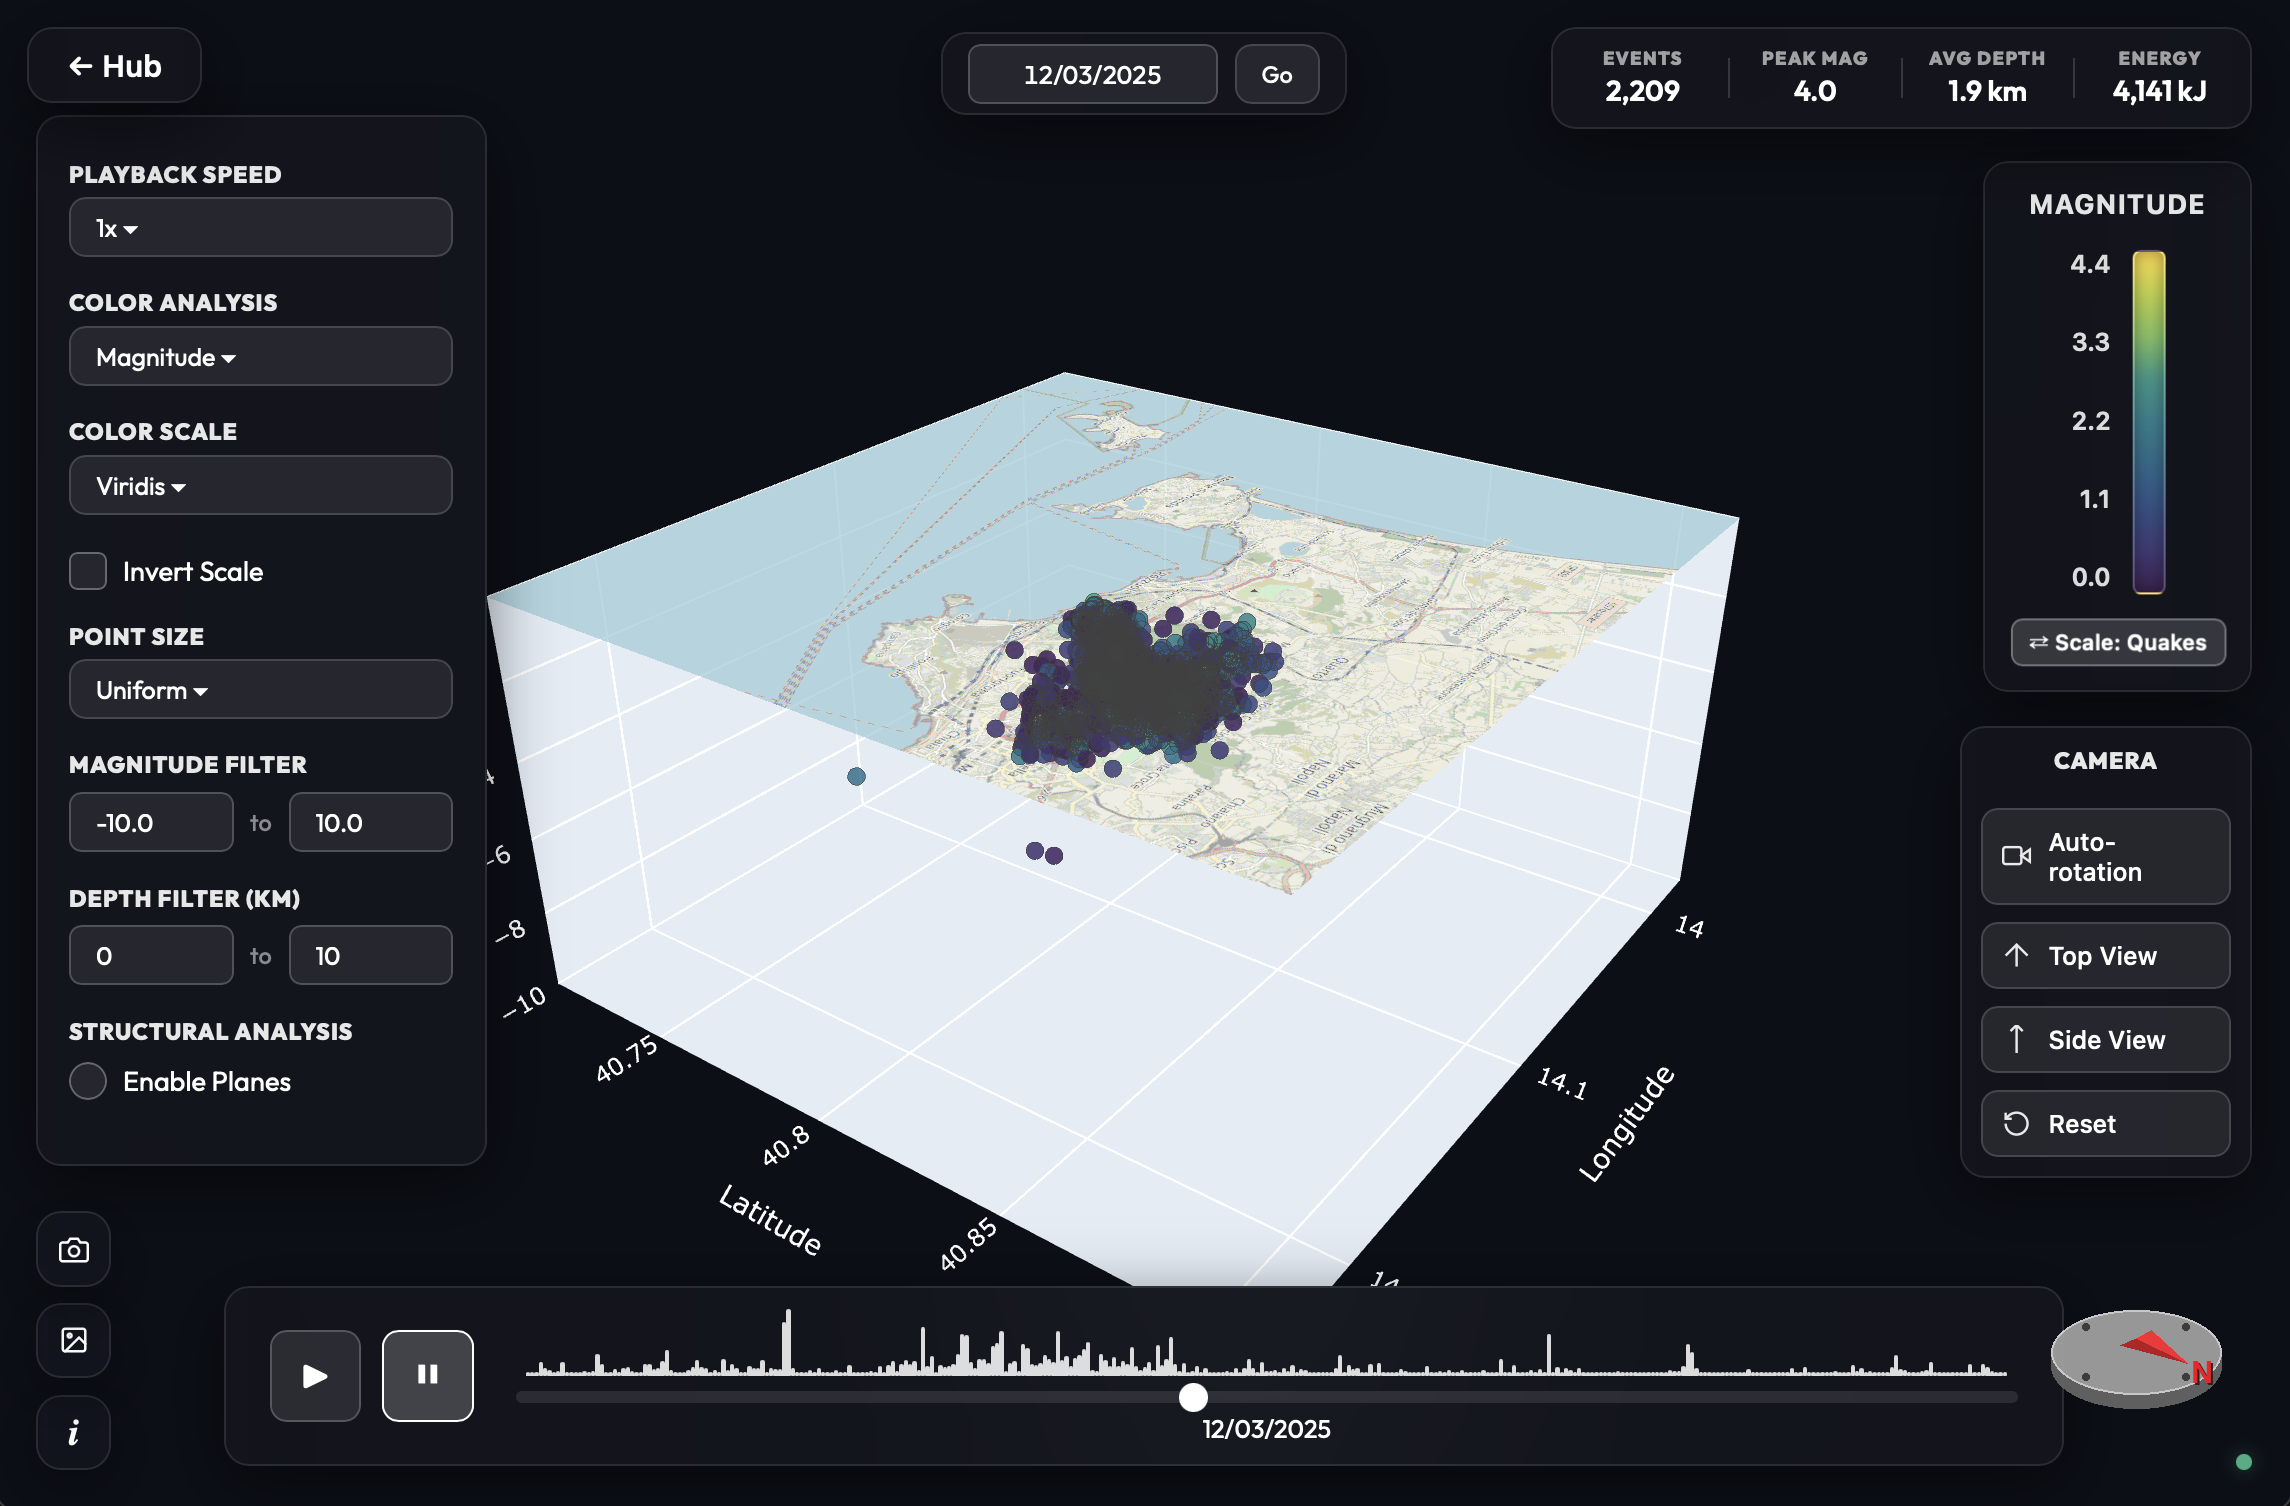
\includegraphics[width=\textwidth]{images/animated_visualization.png}
\caption{Active 4D playback view showing the time-sliced hypocentral point cloud.}
\label{fig:anim-viz}
\end{subfigure}
\end{figure}

\begin{figure}[H]
\ContinuedFloat
\centering
\begin{subfigure}[t]{0.85\textwidth}
\centering
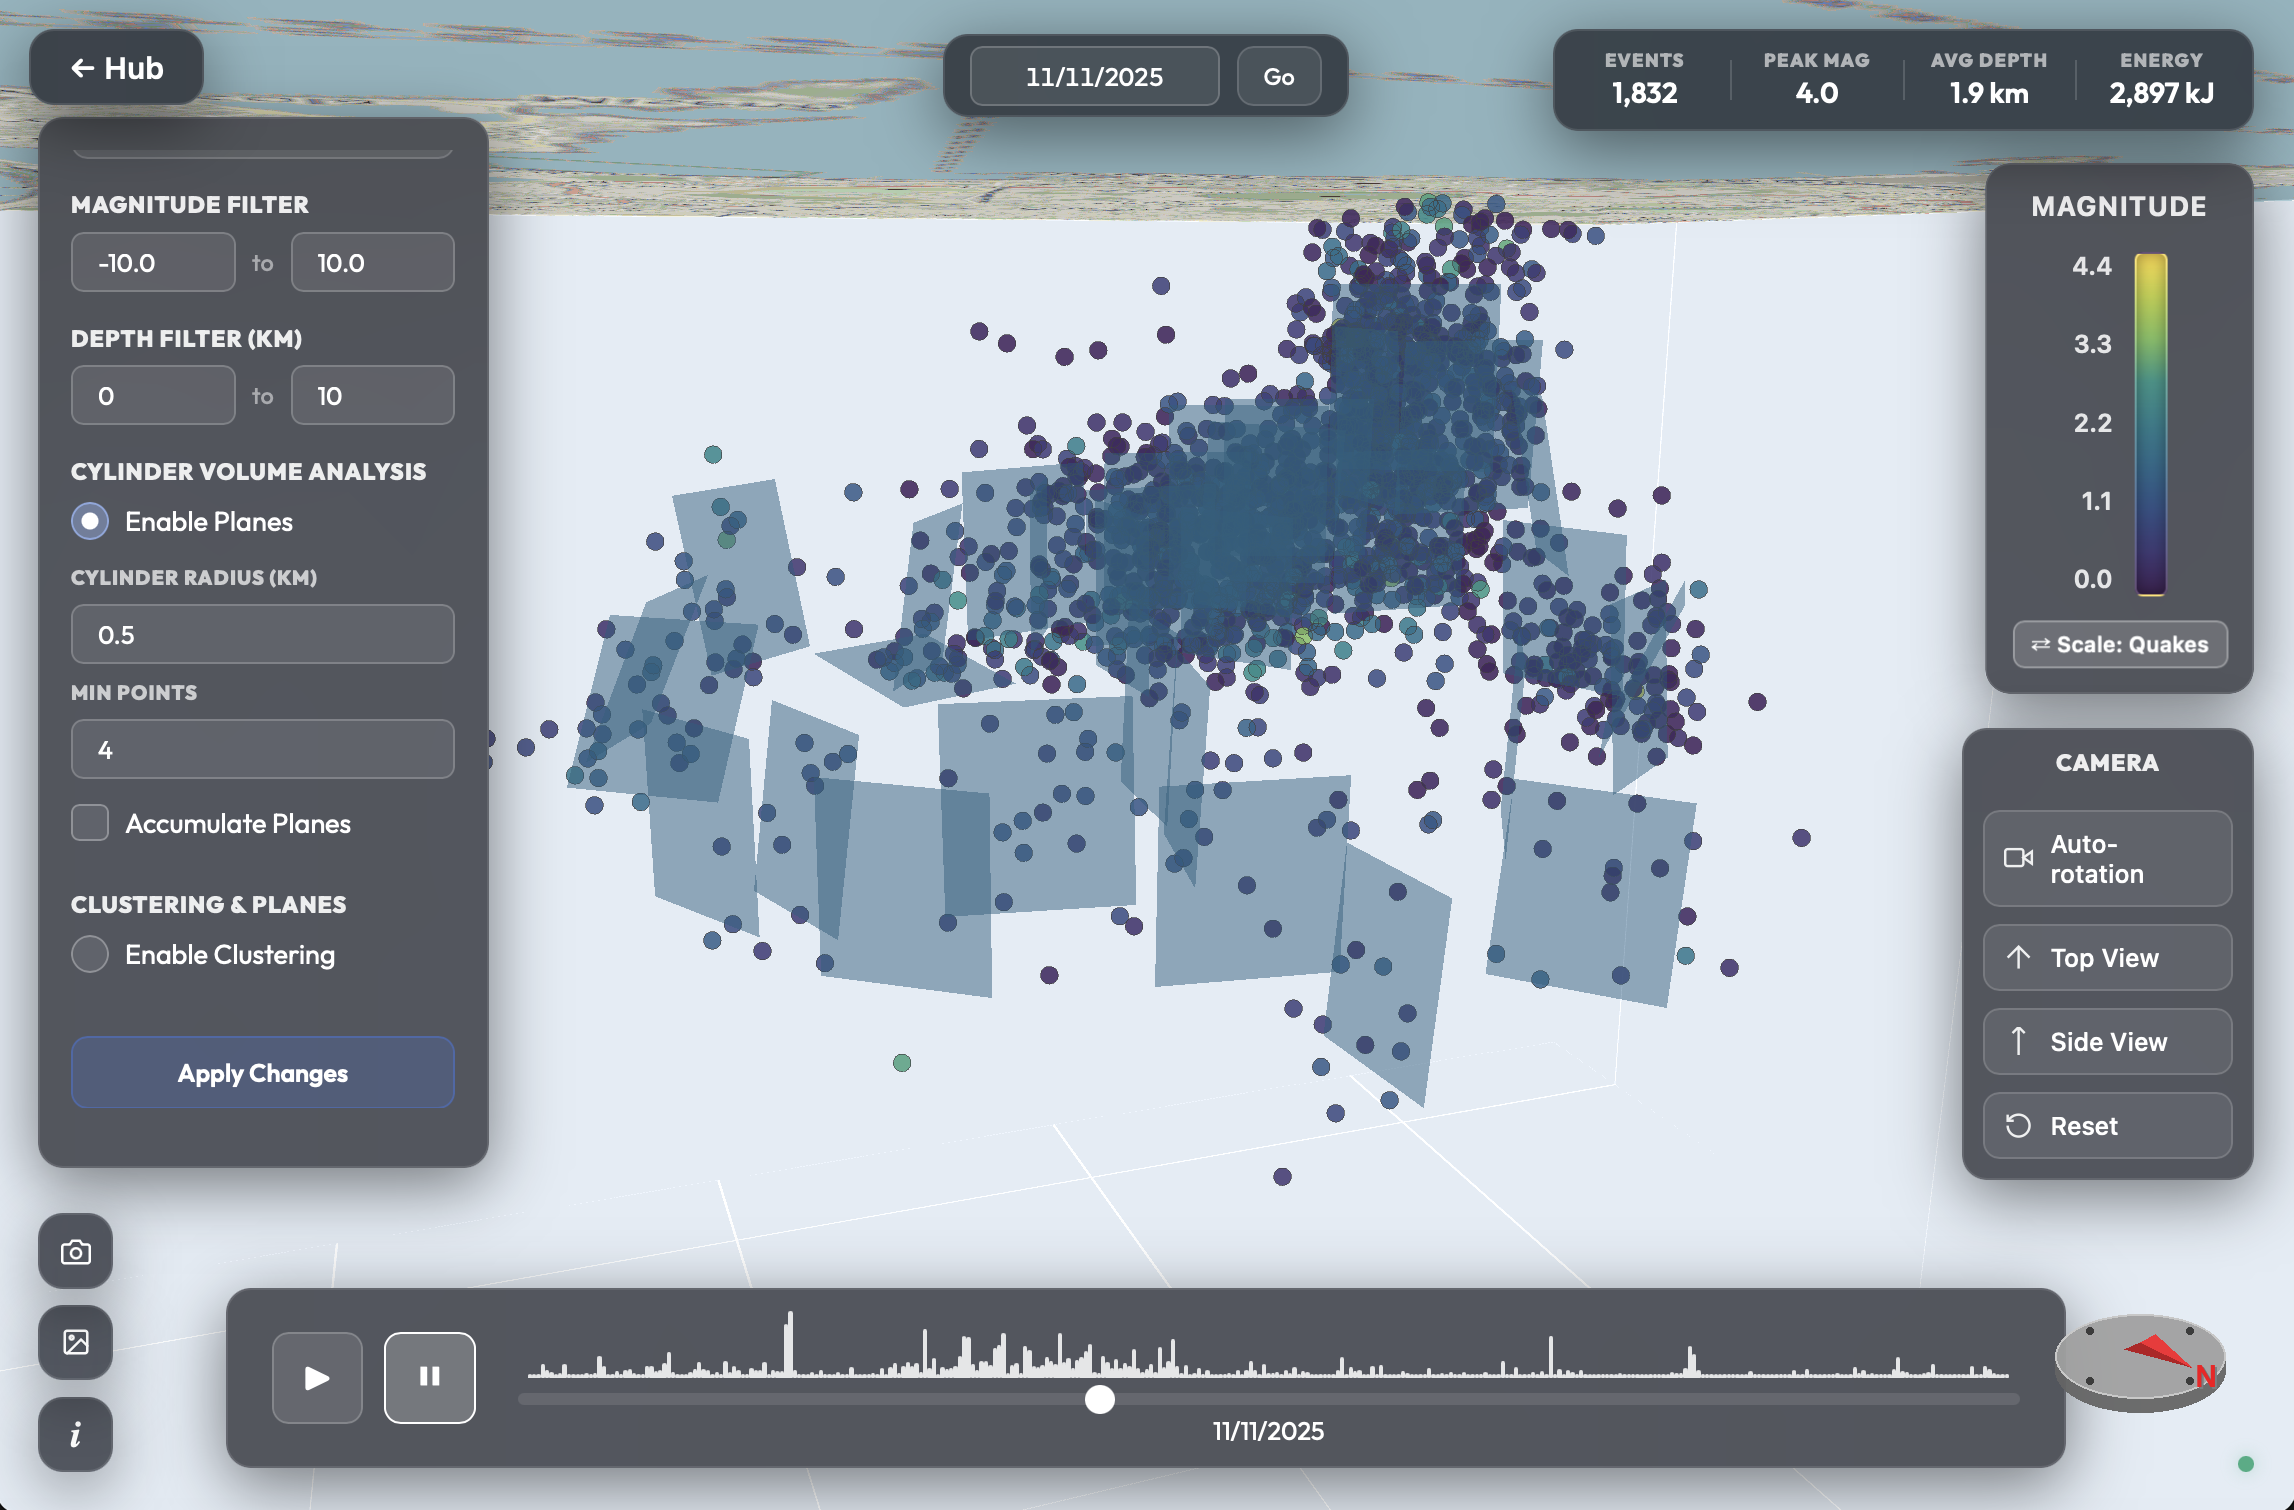
\includegraphics[width=\textwidth]{images/animated_visualization_cylinder_planes.png}
\caption{Dynamic cylinder grid partitioning with automated structural plane fitting during 4D evolution.}
\label{fig:anim-cylinder-planes}
\end{subfigure}
\caption{The 4D Animated Spatio-Temporal View workflow. Users configure parameters via the dialog (\subref{fig:anim-menu}), explore time-evolving seismicity (\subref{fig:anim-viz}), and observe automated fault plane tracking (\subref{fig:anim-cylinder-planes}).}
\label{fig:anim-multi}
\end{figure}

Prior to starting the animation, the time parameters (such as step size and frame rate) are configured via a dedicated dialog window (\Cref{fig:anim-menu}). The resulting 4D view (\Cref{fig:anim-viz}) allows interactive exploration of the chronological sequence. In addition, the volume can be partitioned into a spatial grid of vertical cylinders (\Cref{fig:anim-cylinder-planes}). This subdivision was implemented to better understand the spatial distribution of the data, as partitioning the volume isolates and subdivides the fault geometry into local, simpler planar segments. As earthquakes occur inside these cylinders, the system dynamically calculates and renders these local structural fault planes in real-time, allowing users to visualise how seismic events evolve over time across the identified planar structures.

\section{3D Cluster Analysis View}
\label{sec:view-cluster}

The cluster analysis mode integrates spatial machine learning with structural geological modelling.

\subsection{Cluster Visualisation and Interactive Tuning}

To provide a comprehensive geometrical understanding of seismogenic structures, Seismic Viewer renders every identified cluster through four complementary representations within the 3D WebGL scene. These representations address different analytical needs: boundary delineation, volumetric extent, structural orientation, and individual event membership. Together, they allow researchers to examine a cluster from multiple geometric perspectives simultaneously.
\begin{enumerate}
    \item \textbf{Wireframe Convex Hulls (\texttt{Scatter3d})}: Outer boundary envelopes highlighting the spatial footprint and volumetric extent of each distinct cluster.
    \item \textbf{Triangulated Solid Meshes} (\texttt{Mesh3d}, with \texttt{alphahull=0}): Smooth, semi-transparent volumetric convex hulls enclosing the clusters.
    \item \textbf{Structural Fault Planes (\texttt{Mesh3d})}: Planar surfaces calculated via RANSAC robust estimation coupled with Singular Value Decomposition (SVD) refinement. Each plane displays orientation vectors alongside precise geological strike and dip angles upon mouse hover.
    \item \textbf{Clustered Event Spheres}: Discrete event spheres coloured by cluster label using categorical palettes, with unclustered background noise explicitly assigned neutral grey.
\end{enumerate}
When users interactively adjust spatial clustering hyperparameters, such as neighbourhood radius $\varepsilon$, minimum samples threshold \texttt{min\_samples}, or cluster count $K$, via the side control panel, the frontend dispatches a \texttt{get\_cluster\_update} WebSocket message. The Python backend asynchronously recomputes cluster labels and structural planes without blocking the event loop, returning the newly generated Plotly trace definitions. The frontend then replaces the existing traces in the WebGL scene, thereby updating the visualisation while preserving the user's current camera perspective.

\subsection{Sub-Clustering}
\label{sec:sub-clustering}

To analyse hierarchical structures, researchers can perform secondary sub-clustering on specific data subsets. By utilizing the \textbf{locked clusters} feature, users can preserve previously identified and validated groups. The algorithm will then selectively re-analyse and sub-divide all the remaining unlocked clusters simultaneously. The refined results can subsequently be applied back to merge cleanly into the parent view.

\Cref{fig:cluster-multi} provides an overview of the clustering tools. \Cref{fig:cluster-viz} shows the standard 3D clustering interface. \Cref{fig:anim-clustering-noplanes} displays how clustering evolves over time. To ensure visual consistency, a tracking algorithm guarantees that each cluster maintains the same colour across all animation frames. Finally, \Cref{fig:anim-clustering-planes} and \Cref{fig:anim-clustering-unified} combine the animated clusters with dynamically calculated fault planes and spatial cylinders. This combination allows researchers to observe how geological structures evolve and rotate over time.

\begin{figure}[H]
\centering
\begin{subfigure}{0.95\textwidth}
\centering
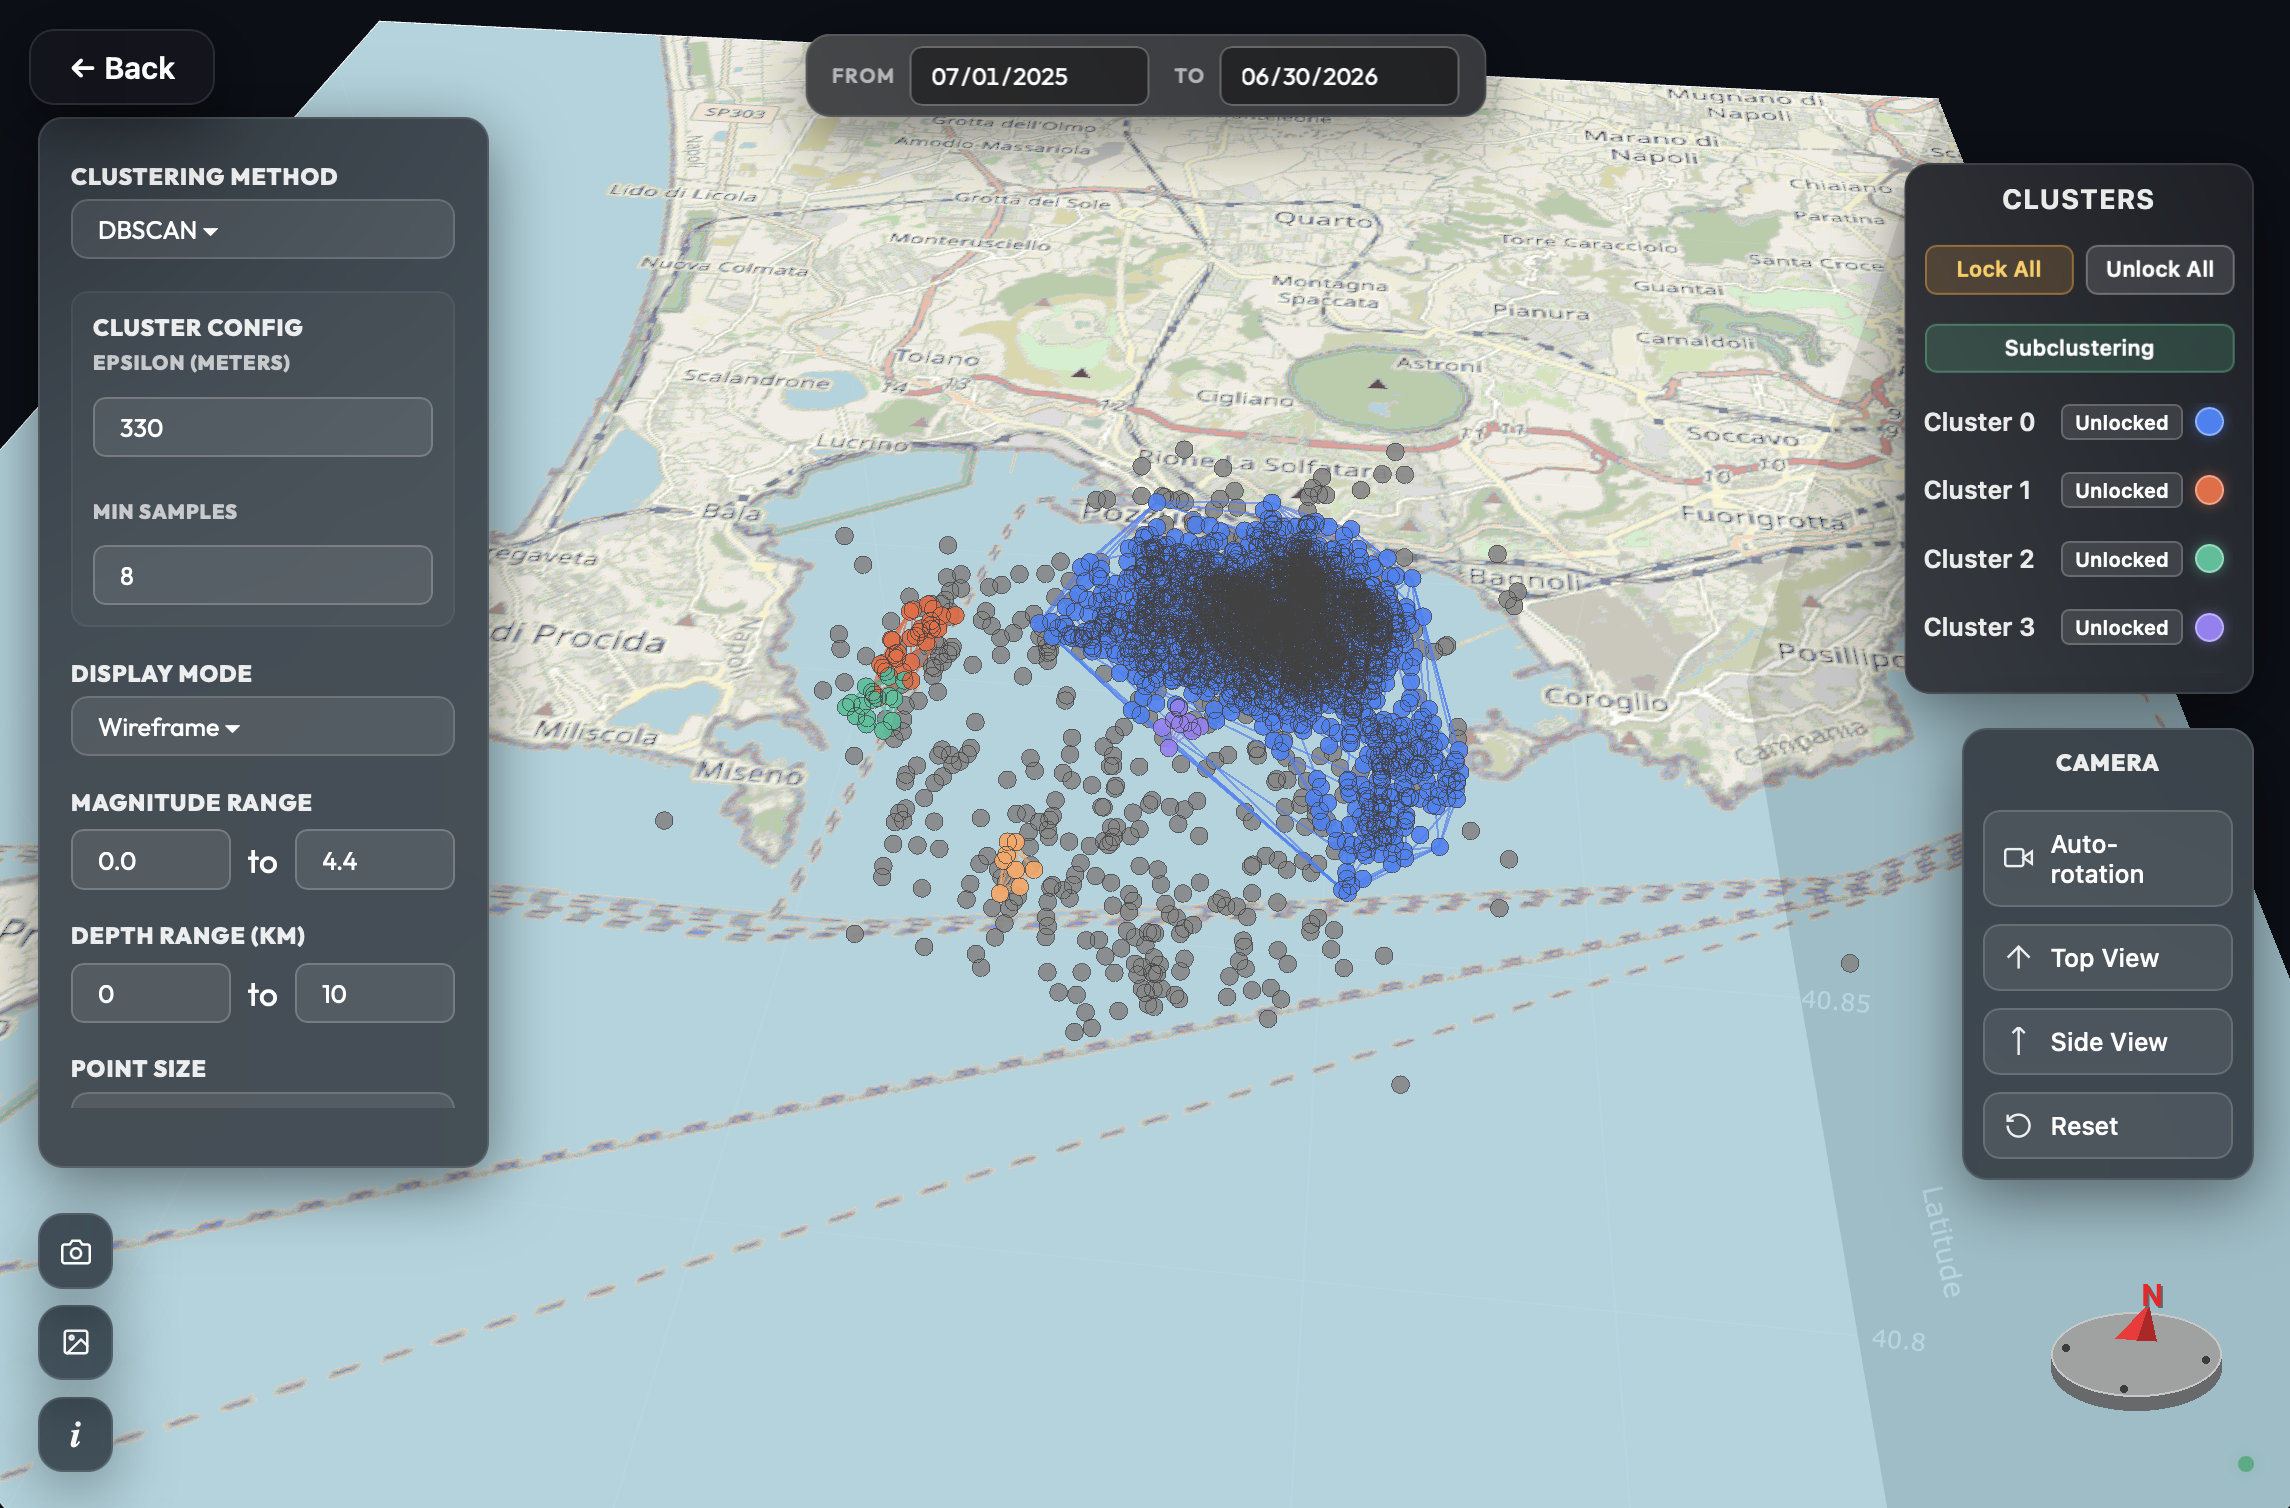
\includegraphics[width=\textwidth]{images/clustering_visualization.png}
\caption{Static 3D workspace with hulls and planes.}
\label{fig:cluster-viz}
\end{subfigure}

\vspace{3mm}
\begin{subfigure}{0.95\textwidth}
\centering
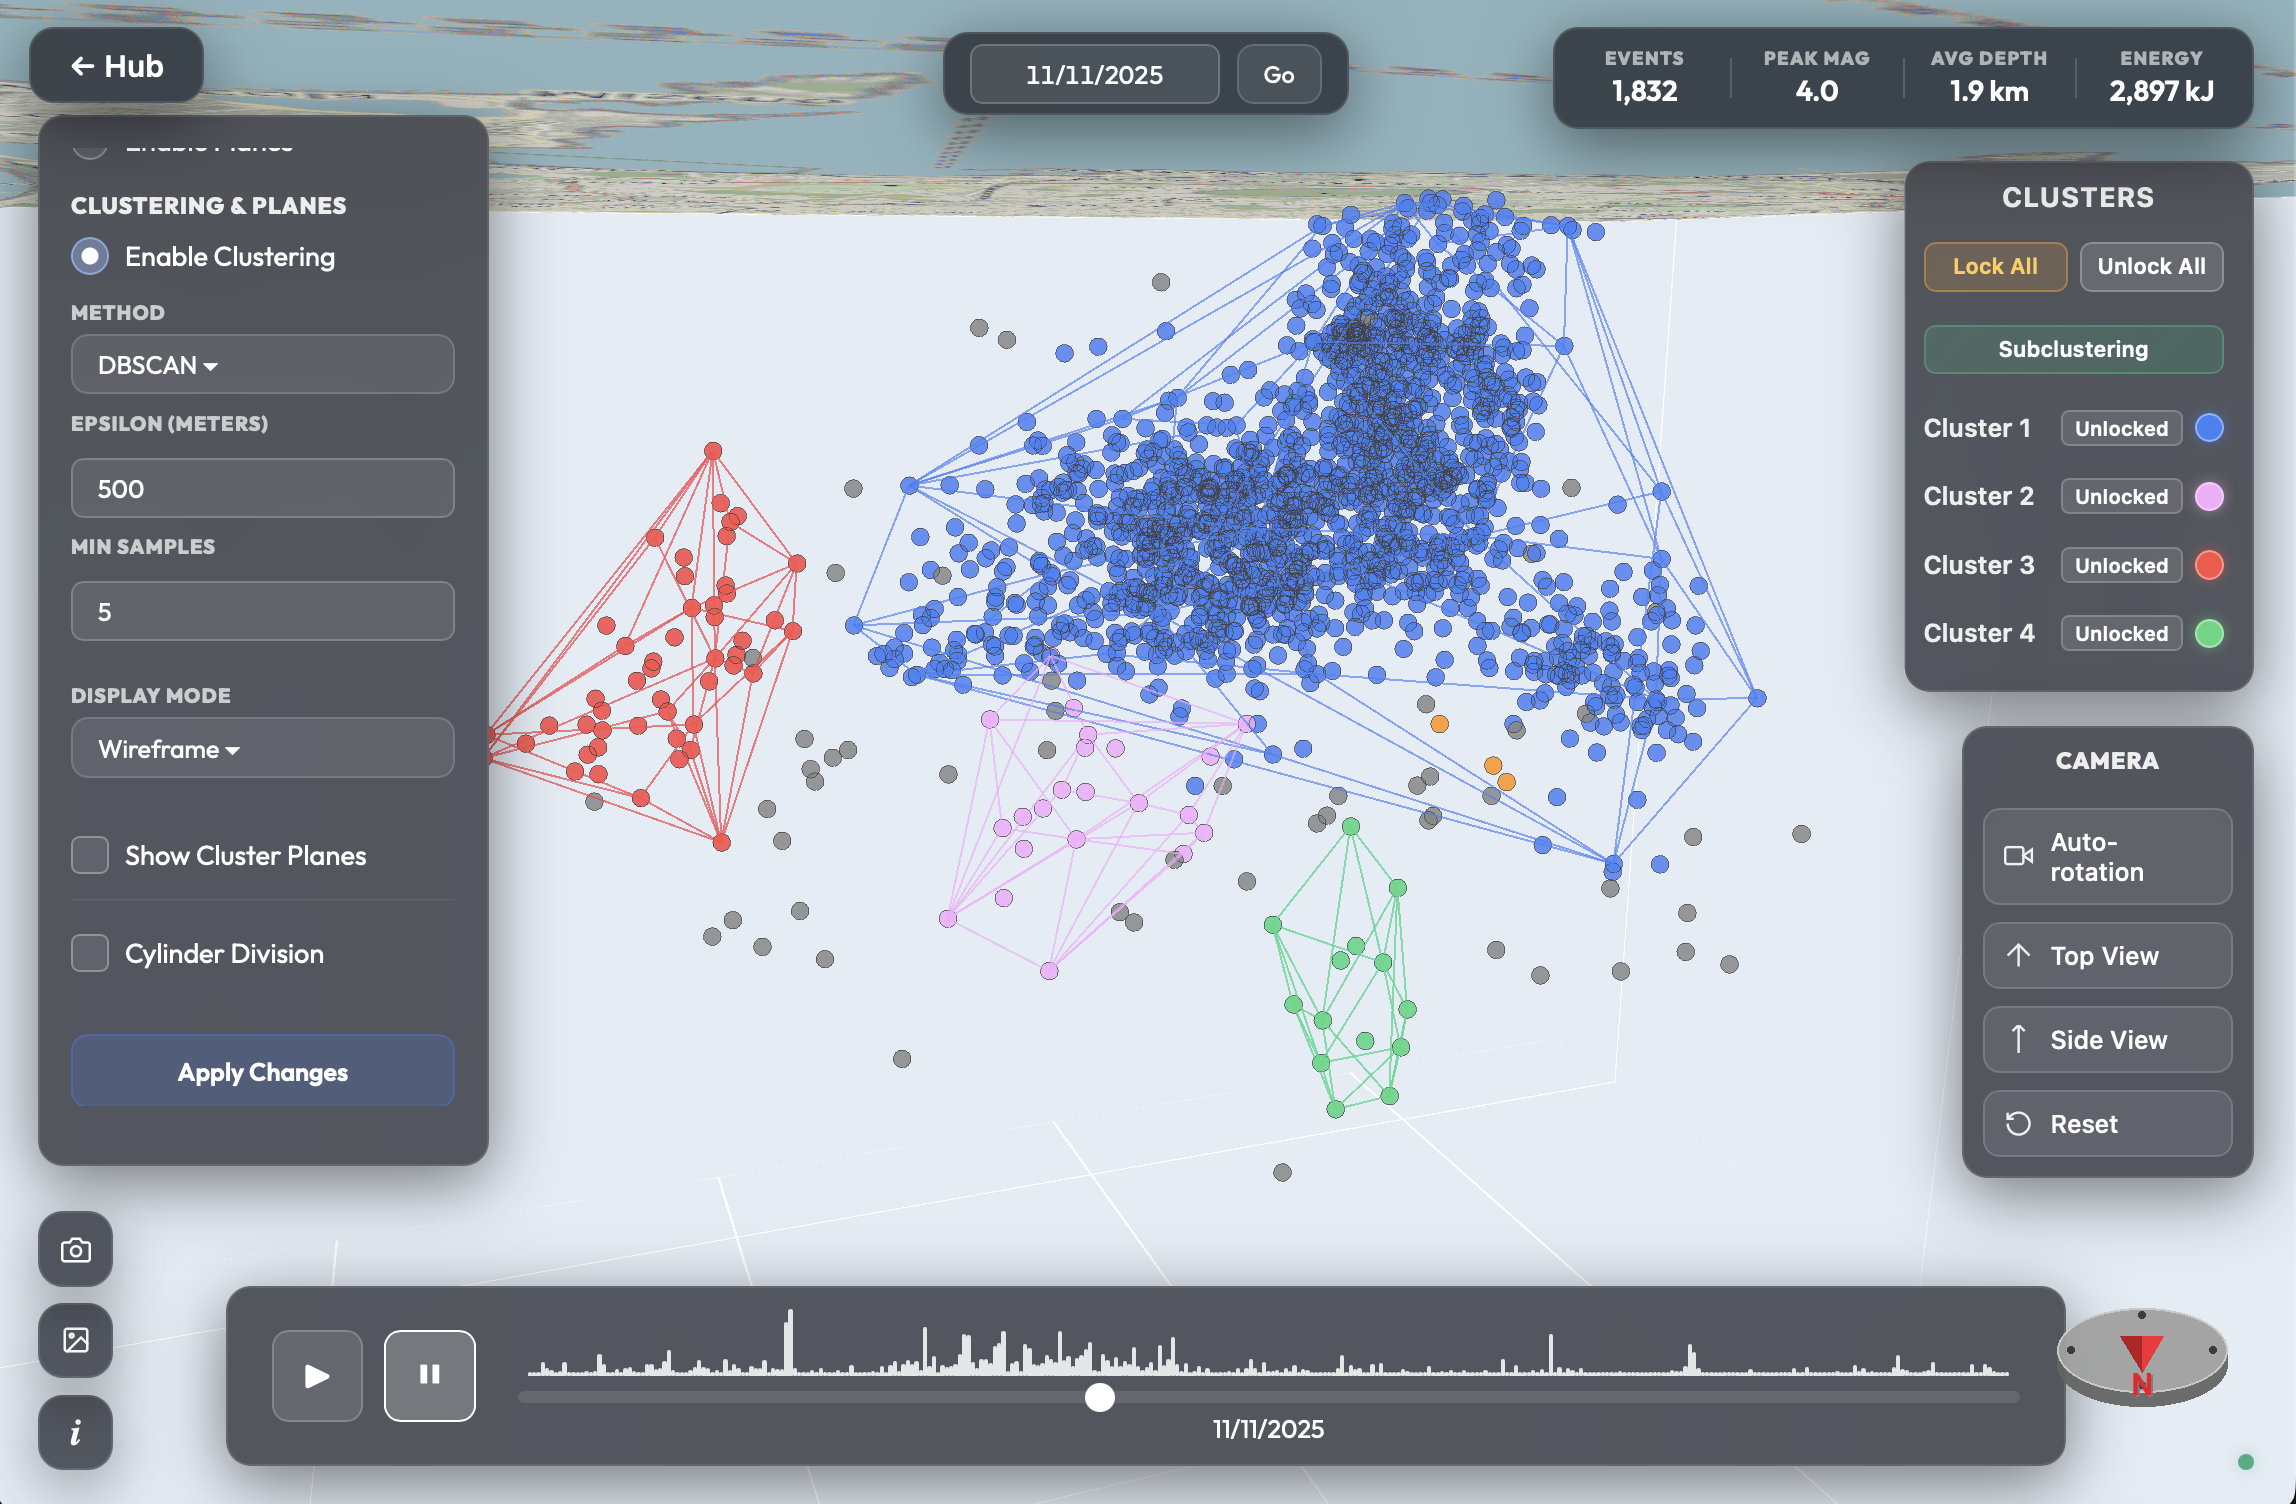
\includegraphics[width=\textwidth]{images/animated_clustering_without_planes.png}
\caption{Animated clustering with Global Label Matching.}
\label{fig:anim-clustering-noplanes}
\end{subfigure}
\caption{Multi-scale static (\subref{fig:cluster-viz}) and animated (\subref{fig:anim-clustering-noplanes} to \subref{fig:anim-clustering-unified}) 3D/4D Cluster Analysis modes (Part 1).}
\end{figure}

\begin{figure}[H]
\ContinuedFloat
\centering
\begin{subfigure}{0.95\textwidth}
\centering
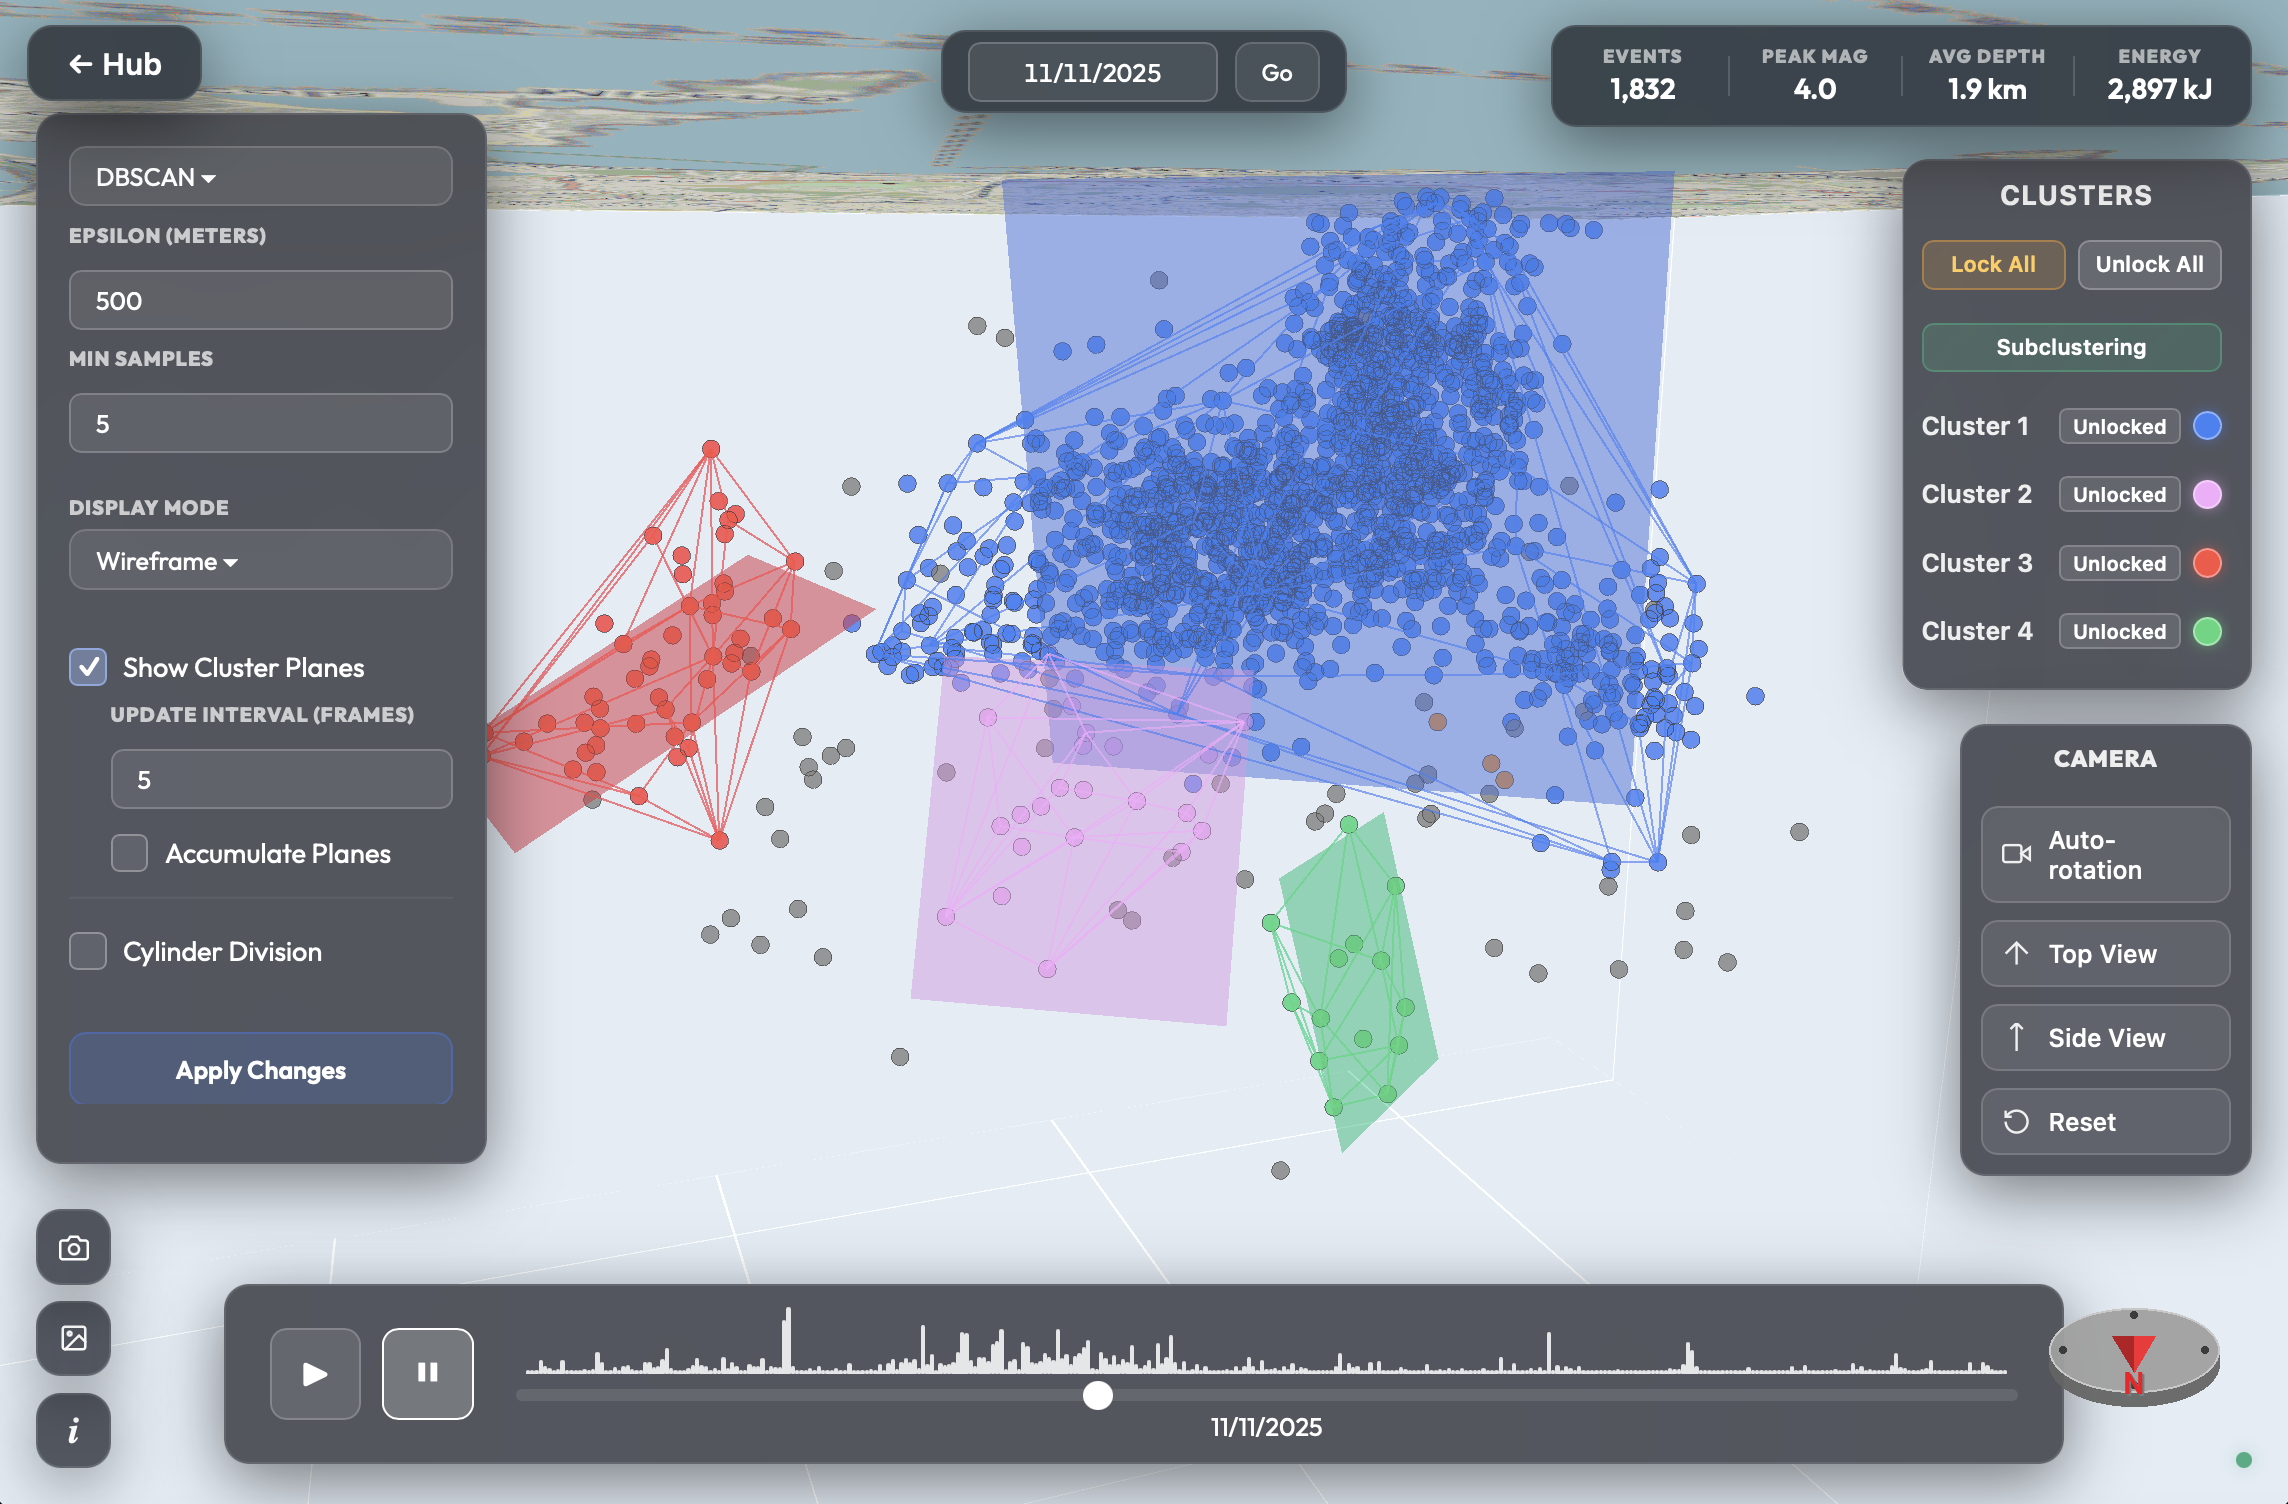
\includegraphics[width=\textwidth]{images/animated_clustering_with_planes.png}
\caption{Animated clustering with RANSAC+SVD planes.}
\label{fig:anim-clustering-planes}
\end{subfigure}

\vspace{3mm}
\begin{subfigure}{0.95\textwidth}
\centering
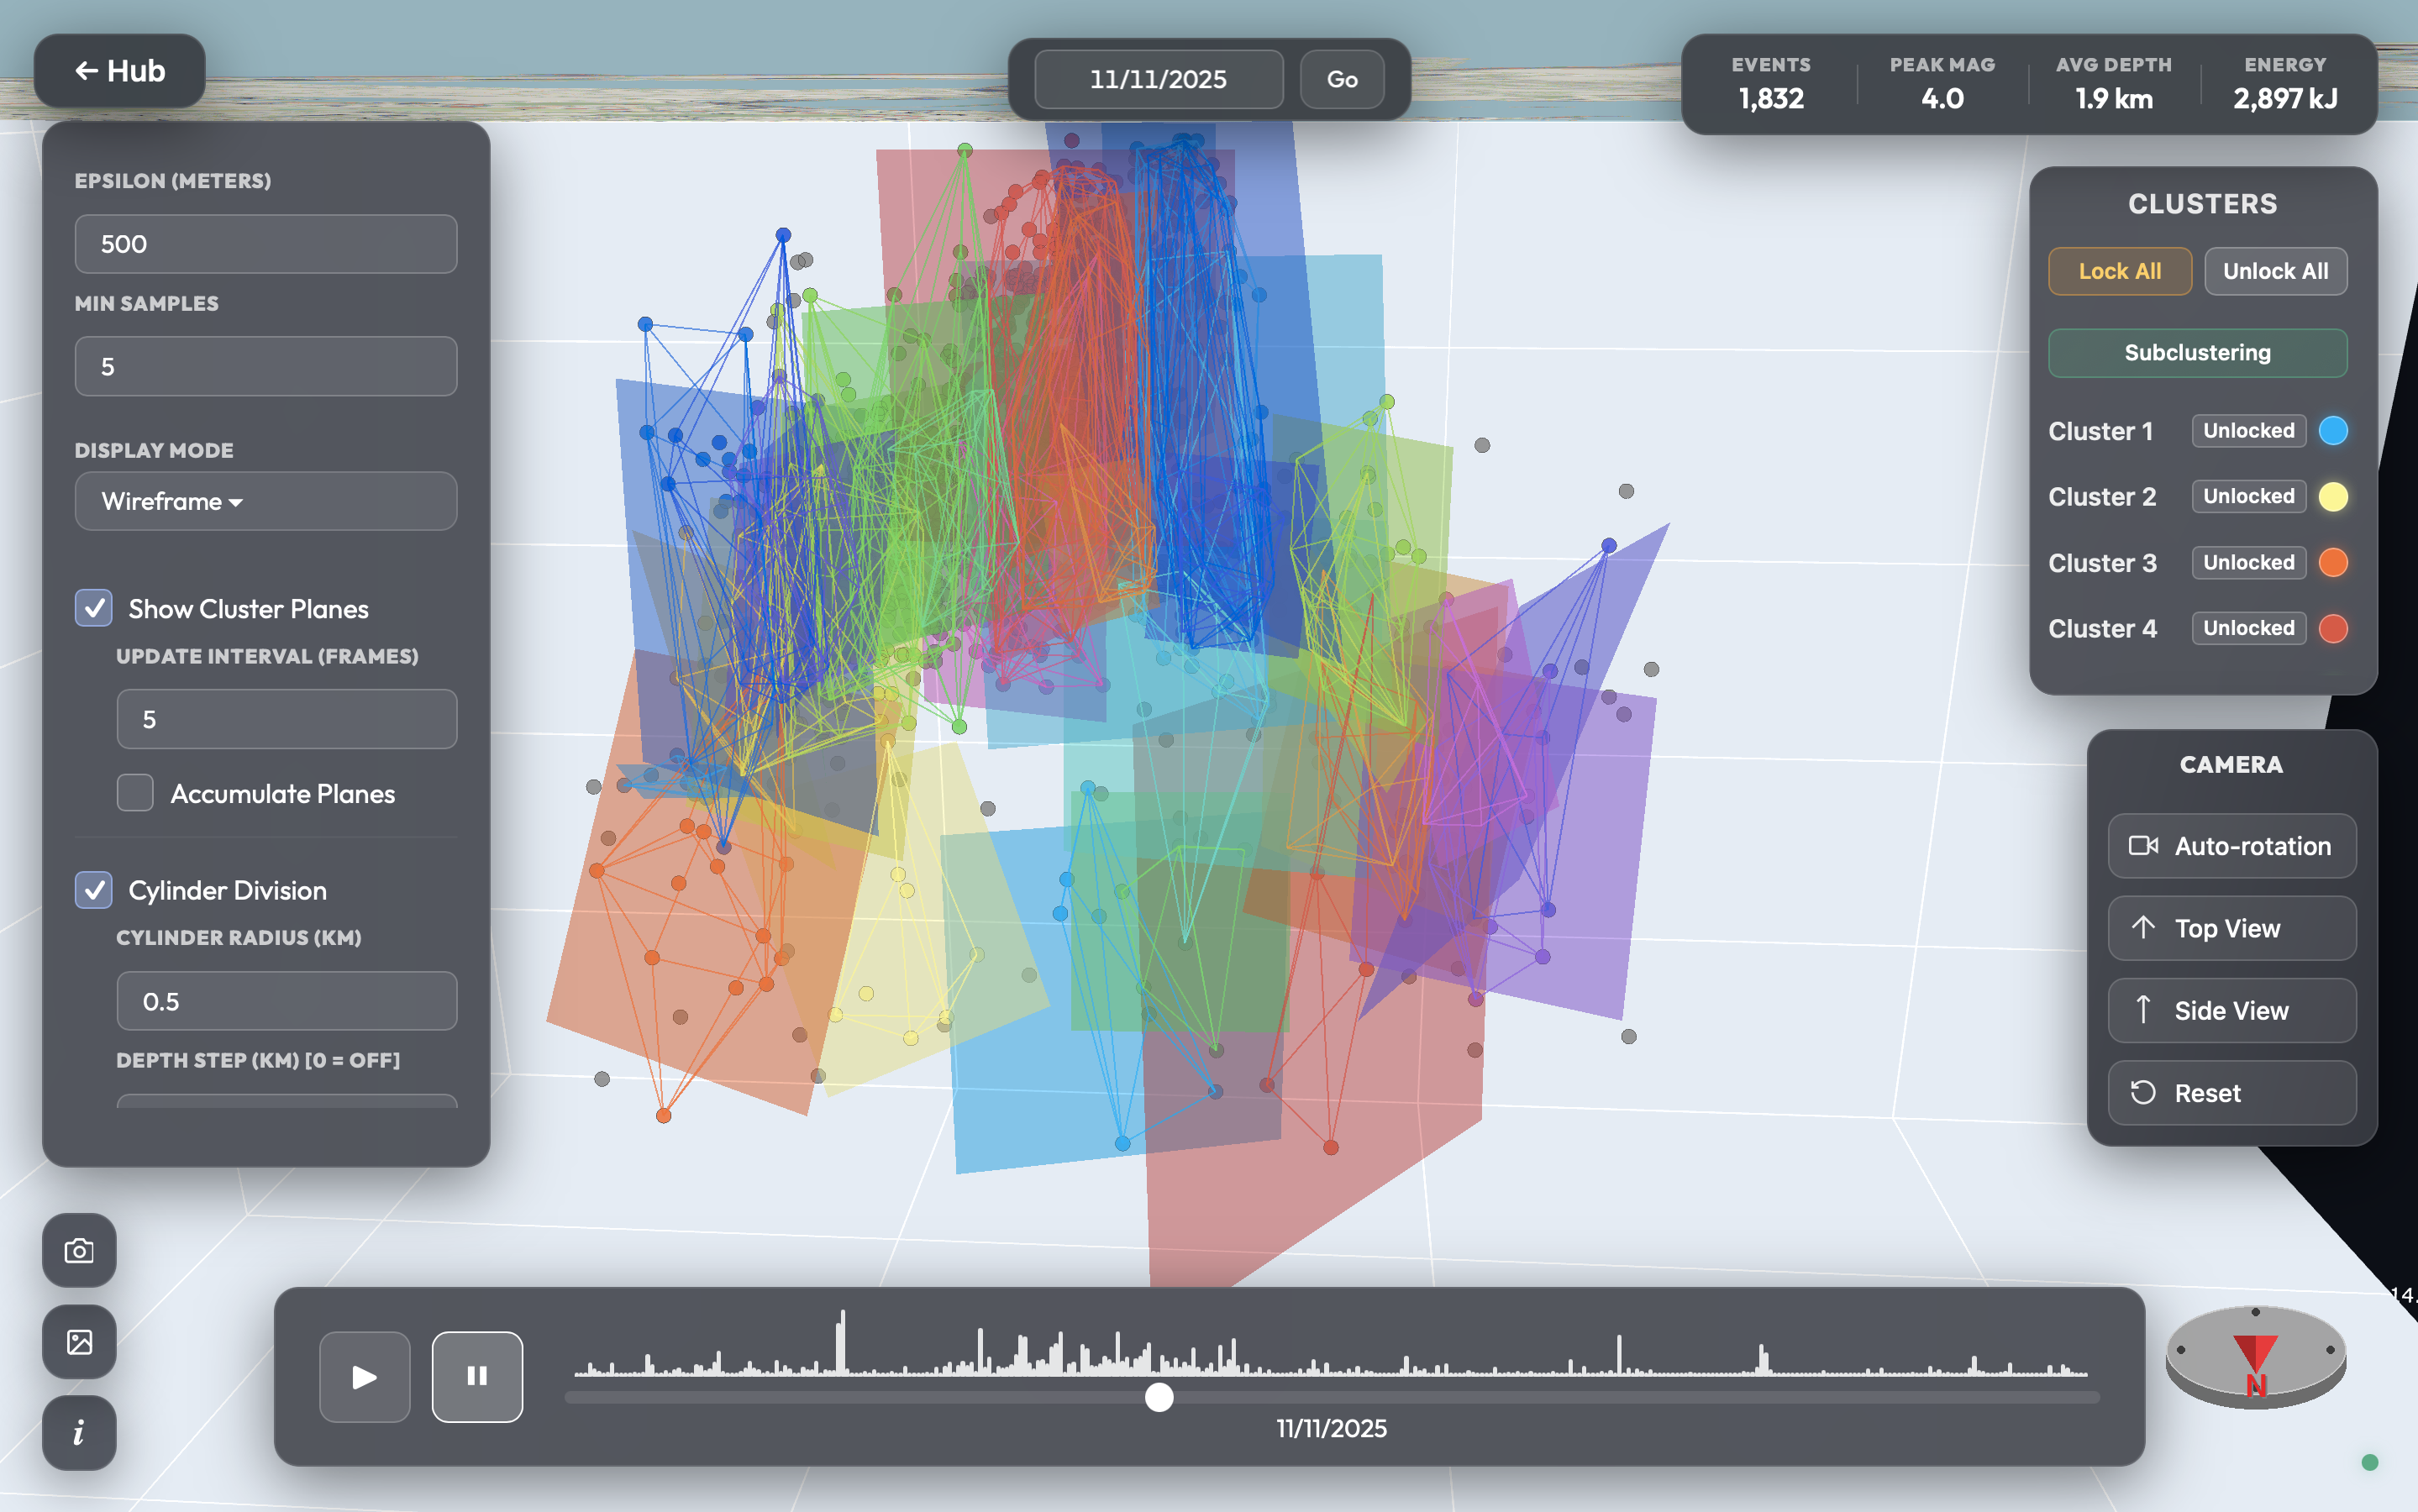
\includegraphics[width=\textwidth]{images/animated_clustering_planes_cylinder.png}
\caption{Unified 4D cylinder partitioning and plane fitting.}
\label{fig:anim-clustering-unified}
\end{subfigure}
\caption{Multi-scale static (\subref{fig:cluster-viz}) and animated (\subref{fig:anim-clustering-noplanes} to \subref{fig:anim-clustering-unified}) 3D/4D Cluster Analysis modes (Part 2).}
\label{fig:cluster-multi}
\end{figure}

\section{Additional Data Layers \& View Caching}
\label{sec:additional-layers}

\subsection{Auxiliary Layers: Tomography, Uplift, and Stations}
\label{sec:tomography}
\label{sec:uplift}
\label{sec:stations}

Seismic Viewer integrates three auxiliary data layers, processed through the \texttt{core/\allowbreak layer\_utils.py} module:
\begin{itemize}
    \item \textbf{Seismic Tomography ($V_p/V_s$ Ratio)}: The raw tomographic data, originally provided in UTM Zone~33N coordinates, is converted to geographic coordinates and projected into physical metric kilometres $(x, y, z)_\text{km}$ using equatorial conversion factors ($k_x = K \cos(\bar{\phi})$, $k_y = K$, depths in km). Because measurements only exist at specific surveyed points, the software estimates values across a regular $30 \times 22 \times 16$ volumetric grid using \textit{Inverse Distance Weighting}. The value of any grid point is calculated as a weighted average of its $k=16$ nearest known neighbours in Euclidean distance ($d$, in physical kilometres), scaling inversely with the square of the distance ($p=2$):
    \begin{equation}
        V(\mathbf{x}) = \frac{\sum_{i=1}^{k} w_i \cdot V_i}{\sum_{i=1}^{k} w_i}, \quad w_i = \frac{1}{d(\mathbf{x}, \mathbf{x}_i)^2}
        \label{eq:idw}
    \end{equation}
    To prevent mathematical artefacts in regions far from observation points, the system applies a distance-decay function. As the distance $d_\text{min}$ (in kilometres) to the nearest station increases, this function smoothly blends the estimated value back into the standard crustal background value ($1.75$):
    \begin{equation}
        V_\text{final}(\mathbf{x}) = \alpha(\mathbf{x}) \cdot V_\text{IDW}(\mathbf{x}) + (1 - \alpha(\mathbf{x})) \cdot 1.75
        \label{eq:gaussian-damping}
    \end{equation}
    where $\alpha(\mathbf{x}) = \exp(-(d_\text{min}/\sigma)^2)$ with characteristic decay radius $\sigma = 2.0$~km acts as the blending weight, decreasing smoothly from 1 (near known data) to 0 (far away), matching the station spacing of the volcanic network.
    \item \textbf{GNSS Ground Deformation (Uplift)}: To visualise ground movement, the system reads historical displacement records and matches them with permanent monitoring stations. To estimate vertical displacement across the entire caldera, the software interpolates values onto a $30 \times 30$ surface grid in metric kilometre coordinates using an IDW weighting exponent of $p=2.5$, modeling the rapid spatial decay characteristic of elastic half-space deformation. The result is displayed on the map either as a coloured 2D surface or as 3D columns rising above the surface.
    \item \textbf{Monitoring Stations}: Permanent station positions are plotted as labelled markers, aiding spatial evaluation of catalogue completeness thresholds.
\end{itemize}

These three auxiliary layers serve complementary roles in the interpretation workflow. By overlaying tomographic anomalies and ground deformation patterns onto the same 3D scene as the earthquake hypocentres, researchers can visually assess whether seismic swarms correlate with known velocity anomalies or with areas of maximum surface uplift, providing a more integrated understanding of the underlying volcanic processes.

\subsection{View Caching and Navigation}
\label{sec:view-caching}

To ensure faster navigation between complex workspaces, the backend bridge maintains an in-memory view cache (\texttt{\_html\_store}, bounded to 4 entries via FIFO eviction) keyed by a composite tuple of file path, view style, animation/windowing parameters, clustering configuration, and locked cluster states. A navigation history stack (\texttt{\_history\_stack}) allows instantaneous back and forward navigation in the clustering view while preserving exact parameter context.

\subsection{Export Engine and Interoperability}
\label{sec:export}

To support external workflows and reporting, Seismic Viewer provides an export subsystem implemented across \texttt{core/exporter.py} and \texttt{assets/viz\_export.js}. Researchers can export filtered catalogues and identified cluster subsets into multiple formats:
\begin{itemize}
    \item \textbf{Structured CSV}: Exports hypocentral coordinates, magnitudes, and timestamps, prefixed with a metadata comment documenting the clustering algorithm and hyperparameters used.
    \item \textbf{GeoJSON}: Formats cluster points into a standard \texttt{FeatureCollection} with geographic point geometries and properties, enabling direct import into external GIS applications such as QGIS.
    \item \textbf{High-Resolution Graphics}: Captures the active WebGL canvas via \texttt{Plotly.\allowbreak toImage}, generating publication-quality PNG renderings.
\end{itemize}
